 \documentclass{article}
\usepackage[utf8]{inputenc}

\title{Approaches for handling missing data in ecological time series}
\author{Modelscapes team\\
}


\usepackage{geometry}                		
\geometry {letterpaper, left=2.5 cm, right=2.5 cm, top=2.5cm, bottom=2.5 cm}    


\usepackage{multirow}
\usepackage{graphicx}		
\graphicspath{ {c:} }
\usepackage{setspace}
\usepackage[version=4]{mhchem}
\doublespace
\usepackage{siunitx}
\usepackage{natbib}
\usepackage{amsmath}
\usepackage{bm}
\usepackage{amsfonts}
\usepackage{lineno}
\usepackage[sharp]{easylist}%makes nice outlines.  Use # for symbol
\usepackage{blkarray}
\begin{document}
\maketitle


\section*{Introduction} 

%%OUTLINE OF THE INTRODUCTION%%
% Older version
% I. Missing data are a common problem in science and can arise in a variety of ways (MCAR, MAR, and MNAR)
% II. Many approaches exist for dealing with missing data from simple deletion/single imputation to more complex, model-based approaches (1-2 paragraphs)
% III. Missing data in ecological settings can present unique challenges.
%   1. Ecological data are often structured as autoregressive time series in which current data partially depend on the value of previous data. In such settings, missing values can be especially problematic as they affect inference on multiple data points.
%   2. Additionally, ecological data can often correspond to non-normal distributions (e.g., count data) that have not been rigorously explored with existing methods of dealing with missing data.
% IV. Here we ....

% New Version (October 2024--feel free to comment!)
% I. Start with there's been a push to collect long term data in ecology, simultaneously with a recent push for rediscovering/analyzing historic datasets (e.g. cherry blossom data). For both scenarios, missingness is common and presents a huge challenge, limiting analyses of large, robust datasets that have been huge efforts to collect.
    % 1. Ecological data collection is particularly prone to missingess because of environmental stochasticity, difficult access, etc.
    % 2. Time series are also more likely to have missingness we can't deal by simply collecting more data, since we can't backfill data at points in time that have already passed. 
 
% II. Missing data in ecological settings can present unique challenges.
    % 1. Ecological data are often structured as autoregressive time series in which current data partially depend on the value of previous data. In such settings, missing values can be especially problematic as they affect inference on multiple data points.
    % 2. Additionally, ecological data can often correspond to non-normal distributions (e.g., count data) that have not been rigorously explored with existing methods of dealing with missing data.
    %3. (very general) There are different types of missigness that can occur in ecological time series (give examples that illustrate the main types of missingess that we include in this MS -- MAR and MCAR w/ different levels of autocorrelation).  
% III. Methods have been proposed for dealing with missing data. However, many were formulated without considering the challenges of missing data in autoregressive time series. While there are some methods that have been developed specifically to address missingness in autoregressive time series, we do not have clear information about how these various methods perform with different types and amounts of missingness and with different types of time series data. 
% IV. Here, we evaluate the precision and accuracy of different statistical approaches for dealing with missing data in autoregressive models of ecological time series data. We test these missing data approaches on real and simulated datasets with both Gaussian and Poisson error distributions. We artificially introduce missingness of different types and increasing amounts into all of these time series, and quantify the performance of different missing data approaches across these three axes of variation in the time series data used (error distribution of the time series, amount of missingness, and type of missingness). This comparison of approaches for dealing with missing data in ecological time series provides a novel comparison of multiple previously-proposed methods of dealing with missing data, some of which have not been previously used with time series data, and will help ecologists determine which method is best suited for addressing the problem of missing data in their particular time series dataset. 

%------------------------------------------

%P1: There's been a push to collect long term data in ecology, simultaneously with a recent push for rediscovering/analyzing historic datasets (e.g. cherry blossom data). For both scenarios, missingness is common and presents a huge challenge, limiting analyses of large, robust datasets that have been huge efforts to collect.
    % 1. Ecological data collection is particularly prone to missingess because of environmental stochasticity, difficult access, etc.
    % 2. Time series are also more likely to have missingness we can't deal by simply collecting more data, since we can't backfill data at points in time that have already passed. 
 
Missing data are a frequent concern in science \citep{rubin_inference_1976, mcknight_missing_2007,allison_missing_2002,little_statistical_2002}, presenting a common challenge in different real-world datasets, including experimental, observational, and meta-analytical data. The problem of missing data is particularly pervasive in primarily field-based disciplines such as ecology, where researchers face many unpredictable environmental barriers to complete data collection\citep{lopucki2022handling, nakagawa_missing_2008}. Datasets with missing observations can arise in many ways, including incomplete data collection due to faulty sensors, inaccessibility of field sites, or even a global pandemic; as well as human error during the data entry or collection processes that necessitates removing observations due to inaccuracy. The consequences of using  data with missing values in subsequent analysis include reduced statistical power \citep{kang2013prevention, moritz_imputets_2017} and biased estimation of parameters, leading to both inaccurate and imprecise conclusions \citep{aleryani2018dealing, kim_transcending_2018, junger_imputation_2015}.% Additionally, missing data typically increase uncertainty, which should be adequately accounted for when confronting models with data \citep{nakagawa_missing_2008,graham_missing_2009}. %AES not really sure what the previous sentence is adding here
Missing data is an acknowledged a problem both within and outside ecological disciplines, yet it is relatively rare that researchers adjust their analyses in statistically rigorous or apposite ways to account for missing observations \citep{nakagawa_missing_2015, junger_imputation_2015, velicer2005comparison}. 

%% P2: Missing data in ecological settings can present unique challenges.
    % 1. Ecological data are often structured as autoregressive time series in which current data partially depend on the value of previous data. In such settings, missing values can be especially problematic as they affect inference on multiple data points.
    % 2. Additionally, ecological data can often correspond to non-normal distributions (e.g., count data) that have not been rigorously explored with existing methods of dealing with missing data.
    %3. (very general) There are different types of missigness that can occur in ecological time series (give examples that illustrate the main types of missingess that we include in this MS -- MAR and MCAR w/ different levels of autocorrelation).  
Perhaps one reason that missing data are often dealt with in a statistically inappropriate manner in ecological analyses is that there are multiple existing tools and workflows for addressing missing data, and their suitability for a given use depends on multiple factors such as the type and amount of missingness, the type of data, and nature of the ultimate analysis \citep{nakagawa_model_2011, hossie_confronting_2021}. %Very small amounts of missing data can be overlooked, while larger amounts must be addressed to preserve model accuracy. %% I don't think we need this sentence, since it's sort of undermining our point...
Per \citet{luengo2010study}, missing $<$1\% of the data is trivial, missing 1-5\% is manageable, and missing $>$5-15\% of the data requires sophisticated handling techniques because it can severely diminish model accuracy \citep{luengo2010study}. Further, data can be Missing Completely at Random (MCAR), Missing at Random (MAR), or Missing Not at Random (MNAR) \citep[][; see Fig.\ \ref{fig:missingtypes}]{rubin_inference_1976}. The MCAR category assumes that the pattern of missing data is independent of the observed and unobserved data \citep{ellington_using_2015, horton2007much}, a rarely tested or valid assumption for empirical ecological datasets due to observer error, collinearity, autocorrelation, and natural variation \citep{nakagawa_missing_2015, hossie_confronting_2021, little_statistical_2002}. The MAR category assumes that missing data are associated with other observed variables but independent of any unobserved or missing variables \citep{newman_missing_2014, ellington_using_2015}. The MNAR category applies to data when the probability of missingness depends on the value of the missing (or unobserved) data. For example, MNAR data occur in ecological time series when sensor accuracy and function are lost during extreme conditions, such as high streamflow, high wind speeds, or low temperatures. Data can be MNAR even if an unobserved variable causes missingness, for example, if streamflow is not measured but high flows cause missingness in another measured variable of interest  \citep{nakagawa_missing_2015}. MNAR assumptions must be specified by the researcher and included during analysis to avoid biased parameter estimates \citep{newman_missing_2014, dong2013principled}. 

These different sources of missingness in datasets lead to different "types" or "mechanisms" of missing data: data are missing completely at random ("MCAR") when missing observations occur in a random pattern in the space or time across which the data were collected, and the occurrence of missing observations in one variable is unrelated to the occurrence of missing observations in another variable (e.g. missingness in the predictor is unrelated to missingness of the response variable); data are missing at random ("MAR") when missing observations occur in a random pattern (as in MCAR), but occurrence of missing observations of one variable is related to occurrence of missingness in another variable (e..g missingness of the predictor occurs at the same time steps as missingness of the response); and data are missing not at random ("MNAR") when the occurrence of missingness in a variable is related to the values of that variable (e.g. a value will not be measured by a streamflow sensor when flow is too high) \citep{nakagawa_missing_2015, gelman_data_2006}.

% p2: Many approaches exist for dealing with missing data from simple deletion/single imputation to more complex, model-based approaches (1-2 paragraphs)

Many methods have been developed to manage missing data and mitigate their impact on statistical analyses (Fig. \ref{fig:ConceptualFigure}). Broadly speaking, these methods can be categorized into simple data processing approaches that occur prior to full statistical analysis or model-based approaches that directly incorporate the missing data into the model-fitting process. The former category primarily consists of data deletion approaches and single imputation. A common example of a data deletion approach is complete case analysis, which, as its name implies, only analyzes complete cases of data while ignoring or omitting cases that contain one or more missing values. However, this approach reduces statistical power and biases parameter estimates \citep{nakagawa_model_2011, aleryani2018dealing}. Rather than removing missing data, single imputation `fills in’ missing data to create complete cases \citep{nakagawa_model_2011} by replacing missing values with either the mean, median, or mode of the data, depending on the data type \citep{kang2013prevention, nakagawa_missing_2015, onkelinx_working_2017}. Although it helps to maximize input, single imputation has received wide criticism due to its failure to consider uncertainty in the imputed values, resulting in overconfident precision \citep{fichman2003multiple, nakagawa_model_2011, aleryani2018dealing}. In contrast to these relatively simplistic methods, several model-based approaches have been developed to directly account for the missing data in the model fitting process. For example, an extension of single imputation, multiple imputation (MI), imputes missing data points many times, resulting in multiple new datasets (\textit{m} datasets) where the imputed values vary stochastically for each missing data point, thus allowing uncertainty to be calculated for parameter estimates \citep{rubin1996multiple, rubin1988overview, nakagawa_model_2011, nakagawa_missing_2015}. In contrast to MI, some model-based approaches use iterative algorithms to handle missing data, either by alternating between parameter estimation and data imputation steps (expectation maximization) \citep{nadjafi2022expectation,li2019expectation, kang2013prevention} or by iterating between predicting and updating steps in time series data (Kalman filter) \citep{kalman_filter_1960}. One more recently developed model-based approach, data augmentation (DA), treats the missing data themselves as unknown parameters to be estimated along with the parameters of a specified model for the data-generating process (e.g., means or standard deviations) \citep{kong_sequential_1994}. While many methods exist for dealing with missing data, not all of them have been adopted for ecological datasets, nor have they been evaluated for their ability to handle missing data in ecological settings.

% p3: Methods have been proposed for dealing with missing data. However, many were formulated without considering the challenges of missing data in autoregressive time series. While there are some methods that have been developed specifically to address missingness in autoregressive time series, we do not have clear information about how these various methods perform with different types and amounts of missingness and with different types of time series data. 

Missing data in ecological settings can present unique challenges.
%   1. Ecological data are often structured as autoregressive time series in which current data partially depend on the value of previous data. In such settings, missing values can be especially problematic as they affect inference on multiple data points.
The nature of ecological data can introduce certain challenges that might exacerbate the presence of missing data. For example, ecological data are often structured as autoregressive time series in which current data partially depend on the value of previous data (e.g., population counts through time or nutrient fluxes within a system). This means that each observation is both a response and a predictor for subsequent observations. In this case, a missing observation could lead to the deletion of multiple data points that depend on it for prediction, resulting in data loss and potentially biased inference. Unfortunately, ecological time series are especially prone to missingness due to a variety of factors including observational errors, sporadic lack of access to field sites, and lapses in funding for data collection. Additionally, the increasing reliance on environmental sensors for ecological data \citep{porter_new_2009} could lead to increased instances of missing data in time series. Sensors often break, lose power, become biofouled, etc., causing a large data loss; this loss can be compounded by infrequent sensor checks due to logistic and financial constraints, resulting in data gaps that last days, weeks, or even months \citep{hossie_confronting_2021}. In fact, due to the COVID-19 pandemic, many more datasets will now have to cope with missing data resulting from field site closures and the disruption of common fieldwork practices due to the necessity of social distancing. Thus, in the context of ecological time series data, there is a need to better understand statistical approaches that can handle gaps in the data, account for the uncertainty imposed by missing data, and acknowledge auto-correlation between present and missing observations. 


Time series with non-Gaussian error distributions are common in ecology and often pose additional modeling challenges. For example, population count data may be modeled using a Poisson or negative binomial distribution, which precludes the use of classical ARIMA models. In these cases, many of the aforementioned model-based approaches for handling missing data must be adjusted to account for the discrete nature of the missing observations. Interestingly, this type of time series has not been confronted with the existing methods of addressing missing data. For example, when using a DA approach, discrete data require exploring discrete parameter space since the missing data are treated as parameters, something commonly-used tools may not be able to handle without additional thought and programming \citep[for example, STAN, a commonly-used software for fitting Bayesian models requires the user to marginalize over discrete parameters in their model specification;][]{carpenter_stan_2017}. While we avoid the technical details here, we aim to illustrate that, with some extra effort, such model-based approaches as EM and DA can be used for incomplete discrete-valued time series.

% p5: Here, we evaluate the precision and accuracy of different statistical approaches for dealing with missing data in autoregressive models of ecological time series data. We test these missing data approaches on real and simulated datasets with both Gaussian and Poisson error distributions. We artificially introduce missingness of different types and increasing amounts into all of these time series, and quantify the performance of different missing data approaches across these three axes of variation in the time series data used (error distribution of the time series, amount of missingness, and type of missingness). This comparison of approaches for dealing with missing data in ecological time series provides a novel comparison of multiple previously-proposed methods of dealing with missing data, some of which have not been previously used with time series data, and will help ecologists determine which method is best suited for addressing the problem of missing data in their particular time series dataset. 

There is limited knowledge of how accurately methods such as multiple imputation or model-based approaches are able to recover parameter estimates or capture the uncertainty imposed by missing data, especially in the context of time series data. Here, we evaluate the ability of multiple methods to recover accurate and precise model parameter estimates and forecast predictions for different amounts and types of missing data. To address this question, we constructed two simple yet realistic time series models for empirical and simulated data, while sequentially removing increasing amounts of missing data and changing the mechanisms of missingness. We deliberately choose mechanisms of missingness that are common in ecological datasets, such as missing data caused by a sensor breaking when temperatures are at extremes or missing multiple successive years in data collection in a long-term population census study. We apply our approach to two illustrative time series models, demonstrating how these methods perform with continuous data containing Gaussian error versus discrete count data with non-Gaussian error. Ultimately, we intend for this comparative study to serve as a resource for ecologists and environmental scientists in search of robust, reproducible methods for confronting time series models with missing data.

[NOT FINISHED YET, WORK IN PROGRESS]

\section*{Methods} 

\subsection*{Overview}

Broadly, we compared the precision, accuracy, and forecasting ability of multiple methods for addressing missing data, using both simulated data and example empirical datasets. We first discuss the two methods we used to generate time series data and our example empirical datasets, followed by presenting the methods for generating different scenarios of ``missingness." Finally, we overview the four different methods of parameter recovery we apply to time series with different degrees of missingness. 

\subsection*{Simulated and empirical Gaussian autoregressive time series models}

%%Overview of our GPP model (mathematical model w/ AR1, light and discharge%

To examine parameter recovery across different missingness scenarios in datasets with Gaussian error, we simulated time series data representative of daily measures of environmental and response variables from a sensor. While this type of time series data is increasingly common in ecological studies and produces high-resolution time series, it is prone to data gaps \citep{chen2013ecological}. We simulated time series data using a first-order auto-regressive (AR1) error model with explanatory covariates, such that:
\begin{equation}
    Y_t = {\bf x}_t'{\bm \beta} + \phi (Y_{t-1} - {\bf x}_{t-1}'{\bm \beta}) + \varepsilon_t
\label{eq:ar1}
\end{equation}
where each time step \(Y_t\) is a function of parameters \(\bm \beta\) and a vector of covariates \({\bf x}_t\), where $'$ denotes the matrix transpose, plus an autoregressive term \(\phi\) times the deviation of the previous time-step from the mean determined by the covariates (i.e. $Y_{t-1} - {\bf x}_{t-1}'{\bm \beta}$). The error term \(\varepsilon_t\) captures both error in this model representation of the variable as well as measurement error, and we assume that $\varepsilon_1, \varepsilon_2,..., \varepsilon_t \overset{iid}{\sim} \mathcal{N}(0, \sigma^2)$ are white noise error terms. For our simulations, we used two covariates and simulated 1000 datasets of 365 observations each, representing a year of continuous sensor data. We note this example could easily be adapted to any number of covariate relationships and alternative autoregressive structures.

% Explain where the Pine River datasets come from %%

We examined forecasting ability against an ecological data set of daily river gross primary productivity (g \(O_2\) \(m^{-2}\) \(d^{-1}\)) across three years, using light (\(\mu\)mol \(m^{-2}\) \(s^{-1}\)) and discharge (\(m^{3}\) \(s^{-1}\)) as covariates \citep{hall_turbidity_2015}. We selected these covariates because gross primary productivity (GPP) in rivers is largely determined by light and flow conditions \citep{bernhardt_metabolic_2018}. Data comes from XXX, providing an almost complete, three year-long time series (n= XXX days for model fitting and YYY days for forecasting comparisons) of gross primary productivity and both covariates.

\subsubsection*{Simulated and empirical Poisson population time series model}

We additionally examined parameter estimation across missingness scenarios using datasets with non-Gaussian error. We simulated time series data of annual counts of individuals in a population using a stochastic Ricker population model \citep{ricker1954stock} such that:

%$$
%\begin{aligned}
%\eta_{t+1} &= N_t \cdot e^{r \cdot \left(1 - \frac{N_t}{K}\right)}\\
%N_{t+1} &\sim f(\eta_{t+1})
%\end{aligned}
%$$

\begin{subequations}
\begin{align} \label{eq:ricker2}
    \eta_{t+1} &= N_t e^{(r - \alpha N_t)}\\
    N_{t+1} &\sim f(\eta_{t+1})
\end{align}
\end{subequations}

\noindent where \(\eta_{t+1}\) represents the expected population size at time \(t+1\), \(r\) is the intrinsic, density-independent growth rate of the population, and $\alpha > 0$ is the intraspecific competitive effect that induces negative density dependence. The population carrying capacity is determined as $K= r/\alpha$. Realized population size, $N_{t+1}$, is a random draw from the distribution $f()$ with mean $\eta_{t+1}$. Throughout our simulations, we set $f()$ to be a Poisson distribution with rate parameter $\eta_{t+1}$, though other error distributions may be appropriate in different empirical applications. We simulated 1000 datasets of 60 observations each, representing 60 years of annual census data. 

Paralleling our above approach, we examined forecasting ability fitting the above Ricker model to a 58-year sequence of annual counts of Great tit (\textit{Parus major}) broods in the Wytham woods in Oxford, UK (CITE DATASET). Census data is continuous from 1960 - 2018. 

\subsection*{Data Missingness Scenarios}

To assess the ability of different modeling approaches to account for differing amounts and types of missing data, we systematically removed observations from both our empirical and simulated time series datasets using two approaches (Fig.\ \ref{fig:missingtypes}). First, for ``missing at random" (MAR) datasets, observations were removed depending on the state of missingness at previous observations, irrespective of the value of the observation (in other words, missingness begets missingness, but is independent of response or covariate values). In contrast, for ``missing not at random" (MNAR) datasets, observations in the lower and upper tails of the response variables were removed, irrespective of the state of missingness in previous sampling events. Motivating these two approaches, for a long-term stream sampling dataset, MAR data might correspond to an individual data logger running out of battery for a few weeks, whereas MNAR data might reflect systematic data logger failures during extreme low or high flow events.

We created MAR datasets with varying proportions of missing data and degrees of autocorrelation in missingness (Fig.\ \ref{fig:missingtypes}B--E) by viewing a time series as a Markov-modulated Bernoulli process where the variable could have two states: missing or not missing \citep{Gharib2014, Edwards1960}. The probability that an observation in a time series at time \textit{t+1} is missing depended on both the specified proportion of non-missing values in the entire time series ($p$) and the specified degree of autocorrelation in missingness ($\omega$). In a time series $X_1, X_2, ..., X_n$, the transition matrix that describes the probability of an observation at $X_{t+1}$ being missing, based on whether the observation at $X_t$ was missing is defined as: 

\begin{equation}
X_{t+1}=
\begin{blockarray}{rcccc}
\text{} & \BAmulticolumn{4}{c}{X_{t+1}}\\
X_t & \text{Present} & \text{Missing}  \\
\begin{block}{r(cccc)}
\text{Present} & 1-(1-\omega)p & (1-\omega)p \\
\text{Missing} & (1-\omega)(1-p) & \omega + (1-\omega)p  \\
[1ex]
\end{block}
\end{blockarray}
\end{equation}



% \begin{equation}
% %\begin{blockarray}{rcccc}
% \begin{blockarray}{rcc}
%  & \BAmulticolumn{4}{c}{\text{X_{t+1}}}\\
% \text{X_t} & Present & Missing \\
% %\begin{block}{r(cccc)}
% \begin{block}{r(cc)}
% Present & $1-(1-\omega)p$ & $(1-\omega)p$   \\
% Missing & $(1-\omega)(1-p)$ & $\omega + (1-\omega)p$   \\
% \end{block}
% \end{blockarray}
% \end{equation}

% Old version, not as equation
% \begin{center}
% \begin{table}[!hbt]
% \begin{tabular}{llll}
%       &                        & \multicolumn{2}{l}{$X_{t+1}$}                             \\
%       &                        & Present               & Missing                                       \\
% $X_t$ & \multicolumn{1}{l|}{Present} & $1-(1-\omega)p$   & \multicolumn{1}{l|}{$(1-\omega)p$}        \\
%       & \multicolumn{1}{l|}{Missing} & $(1-\omega)(1-p)$ & \multicolumn{1}{l|}{$\omega + (1-\omega)p$}
% \end{tabular}
% \end{table}
% \end{center}

\noindent We used this transition matrix to stochastically introduce increasing levels of missingness into both empirical and simulated GPP and population count time series datasets. For each unique time series, we created 150 MAR missing datasets: one for each possible combination of $p$ ranging from 5 to 75\% by increments of 5\% and $\omega$ ranging from 0 to 0.9 by increments of 0.1.  


We created datasets with data missing not at random (MNAR) by removing observations at both the high and low tails of the distribution of observed data (Fig.\ \ref{fig:missingtypes}F,G). These types of MNAR scenarios, where the value of the variable itself is related to its probability of missingness, often occur in data with Gaussian error. However, the MNAR pattern of missingness is unlikely to occur in the population count data with Poisson error because the size of a population in a given year is unlikely to affect the probability of missing data collection that year. (It is important to note that while very low population size may lead to false zeros in a time series of count data, observation error is a problem distinct from missing data). Because of this difference, we only created MNAR missing datasets for simulated and real data with Gaussian error. For each of the simulated AR1 process time series and the empirical GPP time series, we created 15 MNAR missing datasets with $p$ increasing from 5 to 75\% by increments of 5\%. To select observations for removal, we first calculated the mean and standard deviation of the time series with no missing data to create a normal distribution, and then identified the threshold values above and below which the density of the normal distribution corresponded to the desired proportion of missingness. We replaced any values above and below those threshold values with an NA.



\subsection*{Comparing methods of parameter recovery}
We considered several potential approaches for accounting for missing data in the simulated and empirical datasets, including data deletion, multiple imputation, Kalman filter, Expectation Maximization (EM) algorithm, and Bayesian data augmentation (Fig.\ \ref{fig:ConceptualFigure}; see below for more detailed descriptions). For simulated datasets, we fit models using the full time series to assess model parameter recovery relative to true values ($\phi$, $\beta$, and the intercept for AR1; $\alpha$ and $r$ for Ricker). In contrast, we fit empirical datasets with the first 90\% of time steps, and then used the final 10\% to evaluate predictive forecasting performance. 

We compared the accuracy, bias, and precision of parameter recovery within a given data type and missingness type to determine if simulated model approaches behaved varied across different model types (AR1 or Ricker), and to evaluate the effect of type and amount of missingness on model performance. We first standardized parameter estimates ($\frac{\text{modeled param.} - \text{true param.}}{|\text{true param}|}$) so that we could compare precision and accuracy of parameter recovery across parameters and simulated datasets. A standardized parameter estimate of 0 indicates perfect parameter recovery, while a positive or negative standardized parameter estimate indicates positive or negative bias in parameter recovery, respectively. Then, we grouped models first by GPP or population data, then by the missing data approach used (data deletion, multiple imputations, etc.), by the type of missingness in the time series used to fit the model (MAR or MNAR), and by $p$. Finally, we categorized MAR datasets such that $\omega\leq$ 30\% = ``low autocorrelation", 30\% $<\omega<$ 70\% = ``moderate autocorrelation", and $\omega\geq$ 70\% = ``high autocorrelation." Within each of these groupings of models, we calculated the mean and standard deviation of standardized parameter estimates for each model parameter. These means characterize the accuracy (how close to 0) and bias (positive or negative) of each parameter estimate, while the standard deviations characterize the precision of each parameter estimate.  

In each empirical dataset, models were fit to the first 90\% of time steps, and then the resulting model parameters were used to forecast the remaining ~10\% of the time steps (time steps 336-366 in the Pine River GPP time series, and annual values from 2014-2018 in the great tit population size time series). We then compared these forecasts to the observed values for last ~10\% of each time series, and calculated the root mean square error (RMSE) of each forecast. As described above, we then grouped these RMSE values according to the type of data used to fit the model (GPP or population data, MAR or MNAR missingness, $p$, and $\omega$), and then by the missing data approach used. This RMSE value indicates the accuracy with which a model is able to forecast future time steps, with higher RMSE values indicating lower precision and accuracy, and lower RMSE values indicating higher precision and accuracy.     






\subsection*{Methods of recovering parameter estimates}

\subsubsection*{Data deletion}
% State what we did [what pkg did we use for the data deletion?] 
We considered two different data deletion methods. The simple data deletion approach involves removing NA values, compressing the dataset, and running the model as if the time intervals between observations were all equal. We include this method only as a reference since it clearly violates the assumptions of equal spacing between adjacent observations in time. To avoid violating this assumption, the complete case data deletion approach involves removing NAs and any observations that would be predicted by a missing observation (i.e., one time step after an NA). However, those observations are retained in the prediction of subsequent observations.


\subsubsection*{Multiple imputation}

Multiple imputation (MI) is an approach for addressing problems of missing data that systematically fills in NAs with imputed values and creates several different versions of complete data sets.  MI has been used fairly commonly in ecology, with multiple studies evaluating methods and approaches to conduct MI for functional traits \citep{taugourdeau_filling_2014,johnson_handling_2021,penone_imputation_2014}, population biology \citep{onkelinx_working_2017}, time series \citep{hui_gap-filling_2004}, and meta-analyses \citep{ellington_using_2015}.  MI’s effectiveness can depend on the number of imputed datasets (\textit{m}). It is often assumed that \textit{m}=5 is a minimum value \citep{honaker_what_2010}; however, researchers have used \textit{m}=200 when comparing methods in the ecological sciences \citep{onkelinx_working_2017}. In general, larger values of \textit{m} result in more accurate estimates of both parameter values and uncertainty. However, each additional \textit{m} dataset equates to another model that needs to be run, increasing the computation time; this can be particularly problematic for data-rich (e.g., long time series) or complex (e.g., hierarchical) models. After imputing the \textit{m} data sets, the analyses of interest are confronted with each data set, and the estimated parameters from the \textit{m} analyses are averaged using Rubin rules of averaging to get the parameter(s), and associated uncertainty, from which inference can be made. We implemented multiple imputation with the Amelia II package in R \citep{honaker2011}, which uses an EM algorithm (see below) in combination with a bootstrapping technique for deciding what values to impute. 

\subsubsection*{Kalman Filter}

The Kalman Filter was developed to estimate the state of a dynamic system that is observed with error but can be used to derive the likelihood function of a time series with missing observations. To illustrate the approach, assume a state-space model
\begin{equation*}
    \begin{aligned}
        X_t &= \phi X_{t-1} + \epsilon_t\\
        Y_t &= X_t + e_t
    \end{aligned}
\end{equation*}
where $X_t$ is the true ``state" of the system at time $t$, $Y_t$ is the observed value at time $t$, and $\epsilon_t \sim \mathcal{N}(0, \sigma^2)$ and $e_t \sim \mathcal{N}(0, \tau^2)$ are IID white noise error terms for the process and observation error, respectively. The Kalman Filter is primarily focused on estimating the unobserved state of the system, $X_t$, and can be conceptualized as a two-step procedure in which, given an initial state $X_0$, we can forecast the next state $X_1$. Then, following data collection at the next time point, $y_1$, we update the forecast using Bayes' theorem. Specifically, the forecast distribution for $X_1$ is
\begin{equation*}
    p(x_1) = \int p(x_1 | x_0)p(x_0)dx_0
\end{equation*}
where $p(\cdot)$ denotes the probability density function. Assuming IID Gaussian errors, $p(x_1)$ is normal with mean ${\tilde x}_1 = \phi x_0$ and variance $v_1 = \phi^2 \frac{\sigma^2}{1 - \phi^2} + \sigma^2$. Given the observed value $y_1$, we update the estimate of $X_1$ using Bayes theorem
\begin{equation*}
    \begin{aligned}
        p(x_1 | y_1) &\propto p(y_1 | x_1) p(x_1)\\
        &= \mathcal{N}\Bigl(\tilde x_1 + K_1(y_1 - \tilde x_1),\ (1 - K_1)v_1 \Bigr)
    \end{aligned} 
\end{equation*}
where $K_1 = v_1 / (v_1 + \tau^2)$ is the \textit{Kalman gain} and creates a weighted average of the forecast and observation. If the observation error is large, the forecast is favored as an estimate of $X_t$, whereas if the process noise is large relative to the observation error, the estimate of $X_t$ tends towards the observed value $y_t$.
For our focus on missing data, we assume the process is observed without error such that $Y_t = X_t$ and $\tau^2 = 0$. Without observation error, the Kalman gain $K_t = 1$ for all $t$ since $\tau^2 = 0$, and $p(x_1 | y_1) = \mathcal{N}(y_t, 0)$. Thus, the update step gives complete information about $X_t$, and the likelihood function can be defined based on the data $y_1,...,y_n$. However, if data are missing, the update step cannot occur. So, in the case of missing data without observation error, the Kalman Filter alternates between pure forecast steps when data are missing and pure ``update" steps when data and the state of the system are completely observed, but the forecast steps yield a method for computing the likelihood function recursively without needing to know the states of $X_t$ in which we were unable to observe the process and therefore have no associated $y_t$.

Notably, the Kalman filter is the default algorithm used to handle missing values when fitting a time series model with the Arima function in the stats package in R. 

\subsubsection*{EM algorithm}

We used an approximate Expectation Maximization (EM) algorithm to estimate the parameters of the Ricker model in the presence of missing observations. The EM algorithm is an iterative algorithm that is conceptually similar to using the Kalman Filter to recursively compute the likelihood of a time series with missing data. Given an initial guess for the parameter vector we wish to estimate, ${\bm \theta}_0$, the first step (Expectation step) proceeds to ``fill in" the missing observations with their expectation given the observed data and the initial parameter vector ${\bm \theta}_0$. For example, if $Y_t$ were missing, we impute $Y_t$ with $\mathbb{E}(Y_t | y_{t-1}, {\bm \theta}_0)$, which is equivalent to the forecast step of the Kalman filter conditioned on ${\bm \theta}_0$. In the second step (maximization step), we compute the maximum likelihood estimate of ${\bm \theta}$ using the filled-in time series as data to give an updated estimate $\hat {\bm \theta}_1$. We then iterate this process, updating the forecasts of the missing data using their expectations conditional on $\hat {\bm \theta}_1$, then maximizing the likelihood with respect to $\bm \theta$ using the time series filled-in with the updated forecasts. This process is iterated until the difference between successive estimates is acceptably small, indicating convergence (that is, $||\hat {\bm \theta}_i - \hat {\bm \theta}_{i-1}||_1 < \delta$ for some small $\delta > 0$).

We used an approximate EM algorithm to estimate the parameters of the Ricker model in which missing data were rounded to the nearest integer value during the expectation step such that the likelihood was well-defined for the filled-in series. In Figure \ref{fig:EM-bias-checks}, we show that the estimates are asymptotically unbiased. We used the \texttt{optim} function from the \texttt{stats} package in \texttt{R} (v?.?.?) for the maximization step \citep{r_2021}.

\subsubsection*{Data augmentation}

Like the EM algorithm, data augmentation provides a model-based framework for estimating the missing observations as well as the parameters of interest but comes with the added benefit of standard errors for the estimates of all the unknown quantities by treating the missing observations as additional parameters to be estimated. We fit the Gaussian AR(1) models using DA and Stan \citep{carpenter_stan_2017} within R (v?.?.?) \citep{} and using the rstan \citep{} and brms \citep{} packages in RStudio (v?.?) \citep{}. Data augmentation for the population model is not possible with Stan, however (at least not without marginalizing out the discrete parameters, which proved intractable), due to the requirement of continuous parameter space for the Hamiltonian Monte Carlo (HMC) methods Stan uses to sample the posterior distribution. Treating missing integer data as parameters was therefore not possible with Stan, and partially-known parameter vectors are not supported in JAGS. We therefore designed a Gibbs sampler with Metropolis updates for the log growth factor ($r$) and intra-specific competition coefficient ($\alpha$), and Gibbs sampling of any missing observations, $N_{t}^{(0)}$, conditional on $(r, \alpha, {\bf N}_{t-})$, where ${\bf N}_{t-}$ is the vector of abundances (both observed and unobserved) up to but not including time $t$. We used weakly informative Gaussian priors for $r$ and $\ln(\alpha)$ and fit the models using custom functions written in R (v.?). Figure \ref{fig:bias-checks} shows that this algorithm also converges on the ``true" parameter values with increasing sample sizes. 



%\begin{enumerate}
 %   \item Comparing the performance of model approaches for simulated data 
%\begin{enumerate}
 %   \item compare the accuracy of parameter recovery for different methods -- are estimates biased? 
 %   \item compare the precision of different approaches (i.e. average SD for each parameter estimate or 95\% CI across all simulations for each parameter estimate) 
  %  * Q: do we want to do this for all parameters? For just a couple?-- maybe combine fixed effects of light and discharge somehow? 
   % * potentially include the rate at which models fail? (i.e. how sharply does the rate of model non-convergence increase as the amount of missingness increases?)
%\end{enumerate}
%\item Comparing the performance of model approaches for real data 
%\begin{enumerate}
%    \item compare of methods in terms of estimation error (compare forecast RMSE)
%\end{enumerate}
%\end{enumerate}

%* Explain how we did this uniquely for Guassian and Poisson error, for models using MNAR data with increasing amounts of missingness and then for models using MAR data with both increasing levels of missingness and autocorrelation

\section*{Results} 
\subsection*{Time series with Gaussian error}
\begin{enumerate}
    \item MAR data w/ different levels of autocorrelation
        \begin{enumerate}
            \item Results for simulated data
            \begin{enumerate}
                \item accuracy of parameter recovery for different methods (DONE) 
                \item precision of parameter recovery for different methods (DONE)
            \end{enumerate}
            \item Results for real data 
            \begin{enumerate}
                 \item comparison of methods in terms of estimation error (RMSE)
            \end{enumerate}
        \end{enumerate}
    \item MNAR data
    \begin{enumerate}
            \item Results for simulated data
            \begin{enumerate}
               \item accuracy of parameter recovery for different methods (DONE)
                \item precision of parameter recovery for different methods (DONE)
            \end{enumerate}
            \item Results for real data 
                 \begin{enumerate}
                 \item comparison of methods in terms of estimation error (RMSE)
            \end{enumerate}
        \end{enumerate}
\end{enumerate}
%%Bob is splitting results here.  This P should be on method overview
In the simulated AR1 time series with different amounts data missing at random (MAR) and different autocorrelation in missingness (150,000 missing datasets total), our ability to accurately and precisely recover model parameters varied depending on the missing data approach used (data deletion, Kalman filter, multiple imputations, or data augmentation with brms), the amount of missing data, the level of autocorrelation in missingness, and the model parameter in question (Figure~\ref{fig:ParamRec_Gauss}, Figure~\ref{fig:heatMap_gauss_MAR}). Across all MAR simulations, the data augmentation and the Kalman filter missing data approaches recovered model parameters more accurately than other approaches (Figure~\ref{fig:ParamRec_Gauss}: A). The data deletion approach was less accurate, followed by the multiple imputations approach, which in some cases underestimated parameters by over 50\%. 

% P on accuracy of paramater recovery as function of missingness and AC and method
This ranking of missing data approach accuracy was consistent across all levels of MAR missingness, amounts of autocorrelation in missingness, and parameter types. However, the difference between missing data approaches was very small when comparing parameter recovery accuracy for the intercept ($\beta_0$) and the two $\beta$ covariate parameters, as all methods accurately recovered these parameters (within 5\% of the true parameter value) across all levels of MAR missingness and autocorrelation. This similarity was not the case for $\phi$, which was accurately recovered by data augmentation and the Kalman filter across all levels of MAR missingness and autocorrelation, but was increasingly underestimated by models using the data deletion and multiple imputations approaches as the amount of missingness increased. Interestingly, the decline in accuracy of $\phi$ recovery with these two approaches became less steep as the amount of autocorrelation in MAR missingness increased. In other words, we identified a slight trade-off between the effects of amount and autocorrelation of MAR missingness on accuracy of $\phi$ recovery, such that the most inaccurate estimates of $\phi$ came from simulated time series with a high proportion (50\%) and low autocorrelation (0) of MAR missingness (Figure~\ref{fig:heatMap_gauss_MAR}). 

%P on --precision-- of parameter recovery as function of missingness and AC
When comparing across all MAR simulations, precision of parameter recovery typically decreased slightly (or standard deviation of parameter recovery across simulations increased) as the amount of missingness increased (Figure~\ref{fig:ParamRec_Gauss}: B). As with accuracy, all four missing data approaches were similarly precise at recovering the intercept ($\beta_0$) and the two $\beta$ covariate parameters. This precision was generally high and did not vary noticeably across levels of autocorrelation of missing data, but the parameter estimates did become slightly less precise as the amount of missingness increased. Alternatively, all four missing data approaches were less precise when estimating $\phi$, and there was more variation in precision between the different approaches than with the intercept and beta covariates. The relative precision of approaches at recovering $\phi$ was exactly the inverse of their relative accuracy, such that multiple imputations was the most precise, followed by data deletion, and then data augmentation and the Kalman filter, which were very similar. The precision of $\phi$ recovery from models using data augmentation and the Kalman filter tended to decrease as the amount of missingness increased, but that decrease was less sharp as the amount of autocorrelation increased. Precision of $\phi$ recovery for data deletion stayed relatively consistent across missingness and autocorrelation values, while precision for multiple imputations  increased as missingness increased, especially when autocorrelation was high. 

In the simulated AR1 time series with different amounts of data missing *not* at random (MNAR) and different autocorrelation in missingness (150,000 missing datasets total), the accuracy of all methods in recovering $\phi$ and $\beta$ covariates declined substantially (Figure~\ref{fig:ParamRec_Gauss}). Again, data augmentation and the Kalman filter had the highest accuracy in recovering the median standardized estimates for $\phi$ and $\beta$ covariates (though much worse than the MAR data), and multiple imputations had the lowest accuracy in recovering these parameter estimates (Figure~\ref{fig:ParamRec_Gauss}). For all methods, mean standardized estimates for $\phi$ and $\beta$ covariates became increasingly poor at high levels of missingness and tended to underestimate $\phi$ and overestimate $\beta$ covariates (Figure~\ref{fig:ParamRec_Gauss}). For all methods, when data were MNAR, autocorrelation in missingness had no impact on parameter recovery or SD of estimates (Figure~\ref{fig:heatMap_gauss_MNAR}). Similar to the patterns with MAR data, standardized estimates for the intercept were fairly accurate across the range of missingness 
(Figure~\ref{fig:ParamRec_Gauss}). The SD of standardized parameter estimates, especially  $\phi$ were more sensitive to increasing missing data, while the SD of the intercept and the $\beta$ covariates were fairly stable across the range of missing data. 

[Paragraphs about the real GPP dataset]

\subsection*{Time series with Poisson error}

In the simulated Ricker time series with different amounts of data missing at random (MAR) and different autocorrelation in missingness (150,000 missing datasets total), our ability to accurately and precisely recover model parameters varied depending on the missing data approach used, the amount of missing data, the level of autocorrelation in missingness, and the model parameter in question (Figs.\ \ref{fig:ParamRec_Poiss} \& \ref{fig:heatMap_poiss_MAR}). All missing data approaches, on average, overestimated both $r$ and $\alpha$ parameters that were used in the initial Ricker model-based simulations that generated the data. However, some approaches were consistently more accurate than others. The complete-case data deletion and expectation maximization approaches typically recovered model parameters most accurately, regardless of parameter, autocorrelation of missingness, or amount of missingness (Fig.\ \ref{fig:ParamRec_Poiss}A). The data augmentation and multiple imputation approaches were less accurate, with data augmentation performing better in most scenarios. The simple-case data deletion approach was the least accurate, overestimating parameters by close to 80\% in some cases. The amount of missing data, regardless of autocorrelation in missingness, did not strongly affect the accuracy of the complete-case data deletion, expectation maximization, or data augmentation approaches. In contrast, the accuracy of the simple-case data deletion approach decreased markedly as the amount of missingness increased. However, this decrease in accuracy was less substantial as the amount of autocorrelation in missingness increased. We detected a similar pattern in the accuracy of the multiple imputation approach, which became less accurate as the proportion of missing data increased, as long as the missingness had low to moderate autocorrelation. When missing data were highly autocorrelated, the multiple imputation (MI) approach became more accurate as the amount of missingness increased, so that models using MI were able to recover the simulation parameters more accurately when 50\% of data were missing than when the complete dataset was used. It is notable that the missing data approaches we evaluated recovered both $r$ and $\alpha$  with very similar accuracy. 

When comparing across all Ricker simulations, precision of parameter recovery typically decreased slightly (or standard deviation of parameter recovery across simulations increased) as the amount of missingness increased (Fig.\ \ref{fig:ParamRec_Poiss}B). There was not a strong difference in precision of parameter recovery between the $\alpha$ and $r$ model parameters. Whereas different missing data approaches had clear differences in accuracy, most approaches were relatively similar in their precision, especially when estimating the $\alpha$ parameter. Expectation maximization was generally the most precise missing data approach in all scenarios, but especially when estimating the $r$ parameter when missingness was high. Complete case data deletion and data augmentation were the next most precise, and multiple imputation and simple data deletion were the least precise. Two notable exceptions to the pattern of decreasing precision with increasing missingness occurred. First, all missing data approaches recovered the $r$ parameter more precisely in the medium autocorrelation missingness scenario when missingness increased from 0\%  to 10\%. Second, all missing data approaches recovered the $r$ parameter much more precisely in the high autocorrelation scenario when the amount of missingness increased from 40\% to 50\%. 

We also fit Ricker models to 150 versions of a real population time series with different amounts and autocorrelation of data missing at random (MAR), each with the last five observations held out. We used each model to predict the last five years of observations, and found that forecasted population size  was generally quite close to the true value (Fig.\ \ref{fig:forecastAccuracy_poisson}). Forecast accuracy, as measured by root mean square error (RMSE), typically decreased as the amount of missing data increased (Fig.\ \ref{fig:forecastRMSE_poisson}). There was not a clear difference in forecasting ability of models based on the missing data approach that was used. There also was not a clear impact of the amount of autocorrelation of missingness on forecast ability. The one exception to these observed patterns (or lack thereof) is that, for models fit to data with highly autocorrelated missingness using the complete case data deletion missing data approach, forecast accuracy \textit{increases} as the amount of missingness increases. 


\begin{enumerate}
   \item MAR data w/ different levels of autocorrelation
        \begin{enumerate}
            \item Results for simulated data
            \begin{enumerate}
                \item accuracy of parameter recovery for different methods
                \item precision of parameter recovery for different methods (except for EM method, which doesn't return SEs -- but could do 95\% CIs accross all model runs?)
            \end{enumerate}
            \item Results for real data 
            \begin{enumerate}
                 \item comparison of methods in terms of estimation error (RMSE)
            \end{enumerate}
        \end{enumerate}
\end{enumerate}


\section*{Discussion}

\textit{IDEA: an inset box/ sidebar / table with a quick summary of the pros/cons of each missing data approach and recommended + not-recommended data types for each?  Could also incorporate uncertainty generated w. each method, unless that gets too clunky. }

%throughout, talk about the accuracy and precision of each missing data approach (we will add info about forecast accuracy once those results are finished up)

% P1: Our results indicate that missing data doesn't need to be a huge deal, but it is important to choose the appropriate missing data method for your data type and type of missingness
Missing data is a nearly ubiquitous phenomenon in ecological studies and can be particularly difficult when fitting autoregressive time series models since missing values violate the key statistical assumption of equally spaced observations. We evaluated six previously proposed methods for dealing with missing data by fitting autoregressive models to simulated and real examples of two different types of time series common in ecology: daily observations of a continuous variable with a Gaussian error distribution (analogous to sensor data) and annual observations of a discrete variable with a Poisson error distribution (analogous to population size data). Our analyses suggest that missing values in time series do not necessarily have a catastrophic effect on model accuracy, precision, or forecast ability, as long as appropriate steps are taken to account for those missing data so that the basic assumptions of autoregressive time series models are not violated. In fact, models fit using several missing data approaches could recover simulation parameters with relatively high accuracy and precision even when 50\% of observations were missing at random (although we do not suggest fitting models to time series with this much missing data). While we found several missing data approaches that performed well, we did identify some that were uniformly unsuitable. Simple data deletion, where observations that are missing are simply deleted from the time series, led to inaccurate and imprecise models. Multiple Imputation was also quite imprecise, especially for fitting arima models to data with a Gaussian error distribution. However, it is important to consider the type of missingness present in a time series. In time series with Gaussian error with data missing not at random (MNAR), the accuracy of parameter recovery decreased markedly once the proportion of missingness increased above ~10\%.  Below, we delve more specifically into recommendations for missing data approaches for certain scenarios and further explore the impacts of different amounts and types of missing data on model performance. 

\subsection*{For time series, some missing data methods are better than others}

% (P2) Some methods are just not good to use in any scenario
We caution against simple data deletion as an approach to dealing with missing data in time series. While it may be intuitive that simply removing data points could cause irregular timesteps that violate model assumptions, this approach is straightforward and can actually occur under the hood in some modeling packages without it being obvious to the researcher. Parameter recovery after simple data deletion was the worst of all approaches for the population models and second worst for the Gaussian time series. However, if done with care to maintain the autoregressive structure of the dataset through complete case deletion, this approach becomes a viable option depending on the size of your data set and the model's autoregressive structure. With the Ricker model, we effectively regress the population abundance at time $t$ against the abundance at time $t-1$. We, therefore, only need pairs of $(y_t, y_{t-1})$ to estimate $\alpha$ and $r$, which is why the simple complete cases approach worked well under a wide range of simulated conditions. However, if the temporal structure of the model involves longer time lags (e.g., if the population abundance at times $t-k,...,t-1$ for $k > 1$ are all important for the process being modeled), the complete cases approach becomes much less appealing as many more observations become unusable. For example, if we were to consider a model in which we had an endogenous effect of order 2, such that the expected value of $y_t$ depended on both $y_{t-1}$ and $y_{t-2}$, then the observation of $y_t$ would not be usable if either $y_{t-1}$ or $y_{t-2}$ were missing, and only consecutive 3-tuples of data would be usable. This could become limiting with higher order lagged effects or increasing missingness.


% (P3) What is its internal autocorrelation structure of your dataset? What is the type of model you'll be using? What is the error distribution of your dataset? 
   % \begin{itemize}
   %     \item If you have an autoregressive process w several covariates, the Kalman filter may be the best choice. 
   %     \item If Ricker, i.e. each data point only relies on the previous time point, complete case deletion can be one of the best methods. 
   % \end{itemize}


Among the methods that performed well, we found a trade-off in the accuracy and precision of parameter estimation for the Gaussian dataset. Data augmentation and the Kalman filter were more accurate, while multiple imputation and data deletion were more precise for MAR. This finding suggests that ecologists must consider whether accuracy or precision is more important for achieving study objective(s) before choosing a missing data approach (Christie et al., 2019; Fielding and Bell, 1997), though picking one does not necessarily make the other less important. For MNAR, parameter estimates are biased across the methods, with data augmentation and the Kalman filter performing better and multiple imputations performing worse. 


From the Ricker model simulations, complete case deletion and expectation maximization are more accurate and precise in recovering model parameters, indicating the superiority of these approaches over the others for handling missing data. The poor performance of simple data deletion and multiple imputation suggests that these methods are unsuitable for handling missing data at varying levels of autocorrelation and missingness. For instance, simple data deletion overestimates parameter accuracy by ~80\% with increasing levels of missingness and autocorrelation. The consistent and precise recovery of $r$ at medium (with 10\% missingness) and high (40-50\% missingness) autocorrelation levels across the methods highlight the importance of autocorrelation on the precision of parameter estimates. Overall, our results suggest that data augmentation and the Kalman filter are most robust in handling missing data and multiple imputation is the least efficient. It is worth noting that the complexity of a missing data approach is not directly proportional to its efficacy. Data deletion produces poor parameter estimates due to ignoring the linkage between data points. Ecologists should consider Dash and Dash when choosing a missing data approach.

%Of the remaining methods, there are multiple considerations that should inform which missing data method you use. It's important to note that the complexity of a method is not directly related to its efficacy! 



An additional consideration is the type of response variable and whether it is used as an endogenous explanatory variable in the time series model. If the response variable is discrete, data augmentation can be much more difficult to implement and may require custom scripts or clever reformulations of the likelihood that marginalize over the missing observations to fit the model. The expectation maximization algorithm can be easier to implement in these situations, but comes with the drawback of not directly providing standard errors for the estimates. An approach we did not consider here for the integer-valued time series is to use latent (Gaussian) temporal processes to induce temporal autocorrelation in the response variable. Latent temporal process models are common in repeated measures studies that use generalized linear mixed models (e.g., CITE), but these models may not have clear translations from theoretical ecology. Thus, appropriate handling of missing observations in ecological time series data will likely be determined by weighing many practical and theoretical concerns, and there is no uniform solution.


\subsection*{Missing data type matters more than missingness amount with Gaussian time series data}        
%(P4) What type of missingness does the dateset have? (Gaussian example, add Ricker?)

Time series datasets with a large proportion of missing data, up to 40\% had a small effect on parameter recovery accuracy for slope and intercept ($\beta$) terms in the AR1 model using Kalman filter and data augmentation approaches. Estimation of $\phi$ became less accurate as the amount of missting data increased.  Likewise the degree of autocorrelation in the missing data, i.e., the extent to which missing data cluster, had little effect on parameter recovery. In fact, more autocorrelation improved estimates of $\phi$, presumably because consecutive days of measured data are needed to estimate  $\phi$ well.  Indeed high autocorrelation in missingness may make it easier to recover the parameters because having longer uninterrupted stretches of complete data is better than many smaller stretches of data. Overall, the methods used here are quite tolerant of even large amounts of missing  data so long as the data were missing at random (MAR).


The type of missingness affected parameter estimation far more than the amount in terms of correctly interpreting model output and predictions. Perhaps unsurprisingly, parameter estimates and predictive accuracy were generally poorer when data were missing not at random (MNAR; Fig.~\ref{fig:ParamRec_Gauss}). In these scenarios, the missing data introduced a systemic bias to the dataset by removing extreme values and thus artificially constraining the observed variability in the data \citep{rubin_inference_1976}. With MNAR data, $\beta$ parameter estimates diverged greatly with even a small amount (5\%) of missing data. Thus, investigators need to be sure that missing data are due to random events and not a function of the values themselves.  In contrast, when data were missing at random (MAR), no such systemic bias was introduced and all methods performed better and could accommodate higher proportions of missing data (Fig.~\ref{fig:ParamRec_Gauss}). 

Given the strong bias induced by MNAR data, practitioners should first attempt to identify which type of missing data mechanism is at play in their dataset to properly condition their interpretations of model results. Unfortunately, there is no clear statistical test to identify data missing not at random because, by definition, missingness correlates with an unmeasured covariate in the system \citep{van2018flexible}. However, using expert knowledge of ecosystems and data collection methods coupled  with  exploratory data visualizations, one can identify how likely the data are to be missing not at random. For example, if certain monitoring equipment is known to have issues with extreme values or if a histogram of observed data appears highly truncated at the tails (e.g., Fig.\ \ref{fig:missingtypes}G), then it might be more likely that data are missing not at random.  Indeed we suggest caution in assuming that missing data are ever truly random given that e.g., solar powered sensors may fail during dark times of year, sensors biofoul during productive seasons, or population assessments get cancelled due to bad weather.   These scenarios would generate MNAR data in a pattern similar to the simulations here and even small amount of missing data (5\%) could generate biased parameter estimates.  Practitioners should be skeptical of assuming randomness in missing data when interpreting model output regardless of the strategy used to accommodate the missing data.

            %\begin{itemize}
            %    \item MNAR: For the Gaussian data, data that is missing not at random can be a big problem for all of the methods that we tested, often producing very biased estimates with the bias increasing with the amount of data that is missing. --could talk about how to determine whether your data are MNAR? may be practically useful
            %    \item MAR: Gaussian data that is missing at random can often produce decently un-biased estimates, but the confidence in an estimate will decrease with increased missingness. 
            %    \item Ricker examples--type of missingness is not much of a concern, since we really only have one type...
            %\end{itemize}

% (P5) How much data are you missing?
                % \item If you chose a good method of dealing with missing data, and you have MAR data (not MNAR), you can get away with pretty high amounts of missing data (upwards of 30\%!) without sacrificing too much in parameter recovery accuracy and precision.  
                % \item Researchers should consider how much bias they are willing to risk when deciding how much missing data is too much.

 % some studies, e.g. long time series of aquatic metabolism,  Non-random causes could be biofouling during the most productive days of the year, or floods preventing metabolism estimation during the least productive days of the year.

%need to emphasize here and/or at end  that investogators would be wise to not take our word for it, but  to conduct their own fake data simulations, cite Gelman Bayessian workflow)

%(P6) What is the autocorrelation structure of the missingness itself? 
 %           \begin{enumerate}
%                \item  The amount of autocorrelation in your missing data is not as important as how much data you are missing.  
%                \item High autocorrelation in missingness can make it easier to recover the parameters (having longer uninterrupted stretches of complete data is better than many smaller stretches of data).
%                \item Problems with autocorrelated data occur when the missing data stretches coincide with particular conditions in the covariates (aka a type of nonrandom missingness). OR in different words, unless the gaps result in the more systematic missingness in certain covariates that have high autocorrelation.
%                \item Researchers should keep this in mind when designing experiments and anticipating what situations could cause missing data. 
%            \end{enumerate}


% (P7) Parameter recovery bias, in Poisson models in particular 
                % \item E.G. Ricker data: Ricker time series estimates can be especially biased due to low sample size. Population time series data is typically small (<100): it can be difficult to obtain, and therefore has a small sample size compared to other types of data sets. 
               % \item Discussion of how the small sample bias plays out differently across missing data approaches 


 \subsection*{Population models....}
 
Population time series data pose distinct challenges to parameter recovery primarily due to their usually limited sample size. This pattern leads to the problem of small sample size bias in parameter estimation, underscoring the need to select an appropriate method to deal with missing data so as not to further exacerbate this bias. In particular, when fitting discrete population data to a Ricker model with Poisson error without explanatory covariates, the autocorrelation of missingness can substantially affect the results. Data sets with many small gaps (low autocorrelation of missingness), pose greater challenges than data sets with fewer but larger gaps (high autocorrelation of missingness) because parameter recovery depends on the availability of pairs of consecutive non-missing data points, as well as the total number of non-missing data points. In fact, among the methods evaluated, one of the top-performing methods with the least bias was complete case data deletion, where only consecutive pairs of data points are kept, and the rest are deleted. However, caution with data deletion is warranted, as the worst-performing method was simple data deletion, which disregards data gaps and wrongly treats data points before and after a gap as consecutive points. Expectation maximization ties complete case data deletion for the best method for this data type, with multiple imputation and data augmentation giving estimates with intermediate bias.



\section*{Considerations for choosing how to account for missing data}

% (P8) What information from the models do you plan to use? Do you want the model parameters only, or do you also want estimates of the actual data values that were missing? Some approaches can provide both, while others can only provide the former. 
Selecting a missing data approach depends on the goals of data analysis. All of the methods we present are useful in generating parameter estimates based on a model describing the data; however, not all of them generate estimates of the missing data values. If such estimates are desired, data augmentation, which treats the missing data points as parameters, and multiple imputation, which imputes several versions of the dataset, can provide estimates of missing response variables. Additionally, either of these methods could be adapted to accommodate missing values in predictor variables if a model for those data was incorporated. While both approaches will provide an estimate of the uncertainty for the filled-in data points, this interval may be more robust for the data augmentation than multiple imputations which will be influenced by the number of imputations used. Both the Kalman filter and expectation maximization algorithms forecast or impute across data gaps without estimating each step, and thus cannot generate estimates of the missing data. Data deletion approaches, of course, do not provide a filled-in dataset as part of the results. 


%(P9) Comparison to what other missing data papers have found 
%        \begin{enumerate}
%             \item Are we confirming, contradicting, or adding to the available literature on best practices in dealing with missing data?
 %       \end{enumerate}


Our simulations showed that under certain conditions, parameter estimation is robust to high levels of random missingness.  On the surface this finding is useful, but may not be universal to the myriad ecological time series applications that inevitably have missing data. Investigators would be wise to verify the effects of missing data for their own situations and models by conducting tests as we have done here with simulated missing data. Indeed such simulated data exercises are a necessary part of the modeling workflow \citep{gelman2020bayesian}.  

\subsection{Conclusion}
Big take home message: Missing data don't have to be a big problem! Even with half of your dataset missing, using the correct approach to dealing with the missingness can result in decent parameter estimates.    


\newpage


\section*{Figures}

\begin{figure}[h]
    \noindent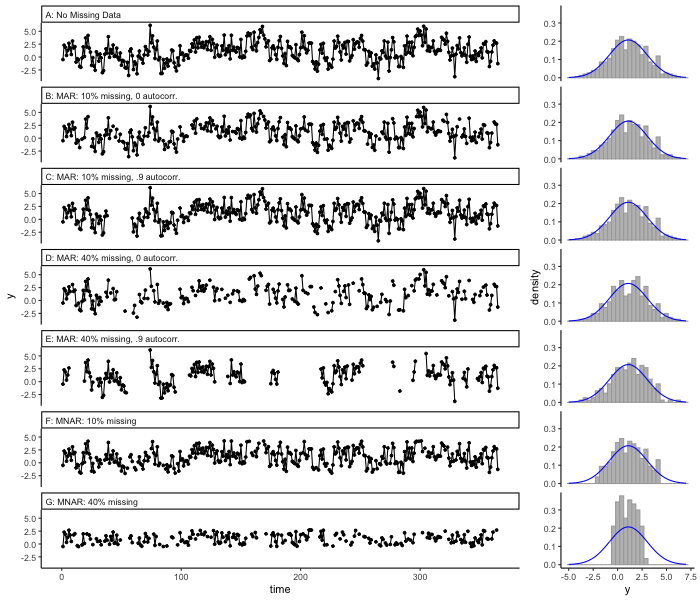
\includegraphics[width = 0.9\textwidth]{Figures/CompareMissingnessTypes_fig.png}
    \caption{Example of a AR1 time series with different proportions and types of missing data}
    \label{fig:missingtypes}
\end{figure}

 
\begin{figure}[h]
     \noindent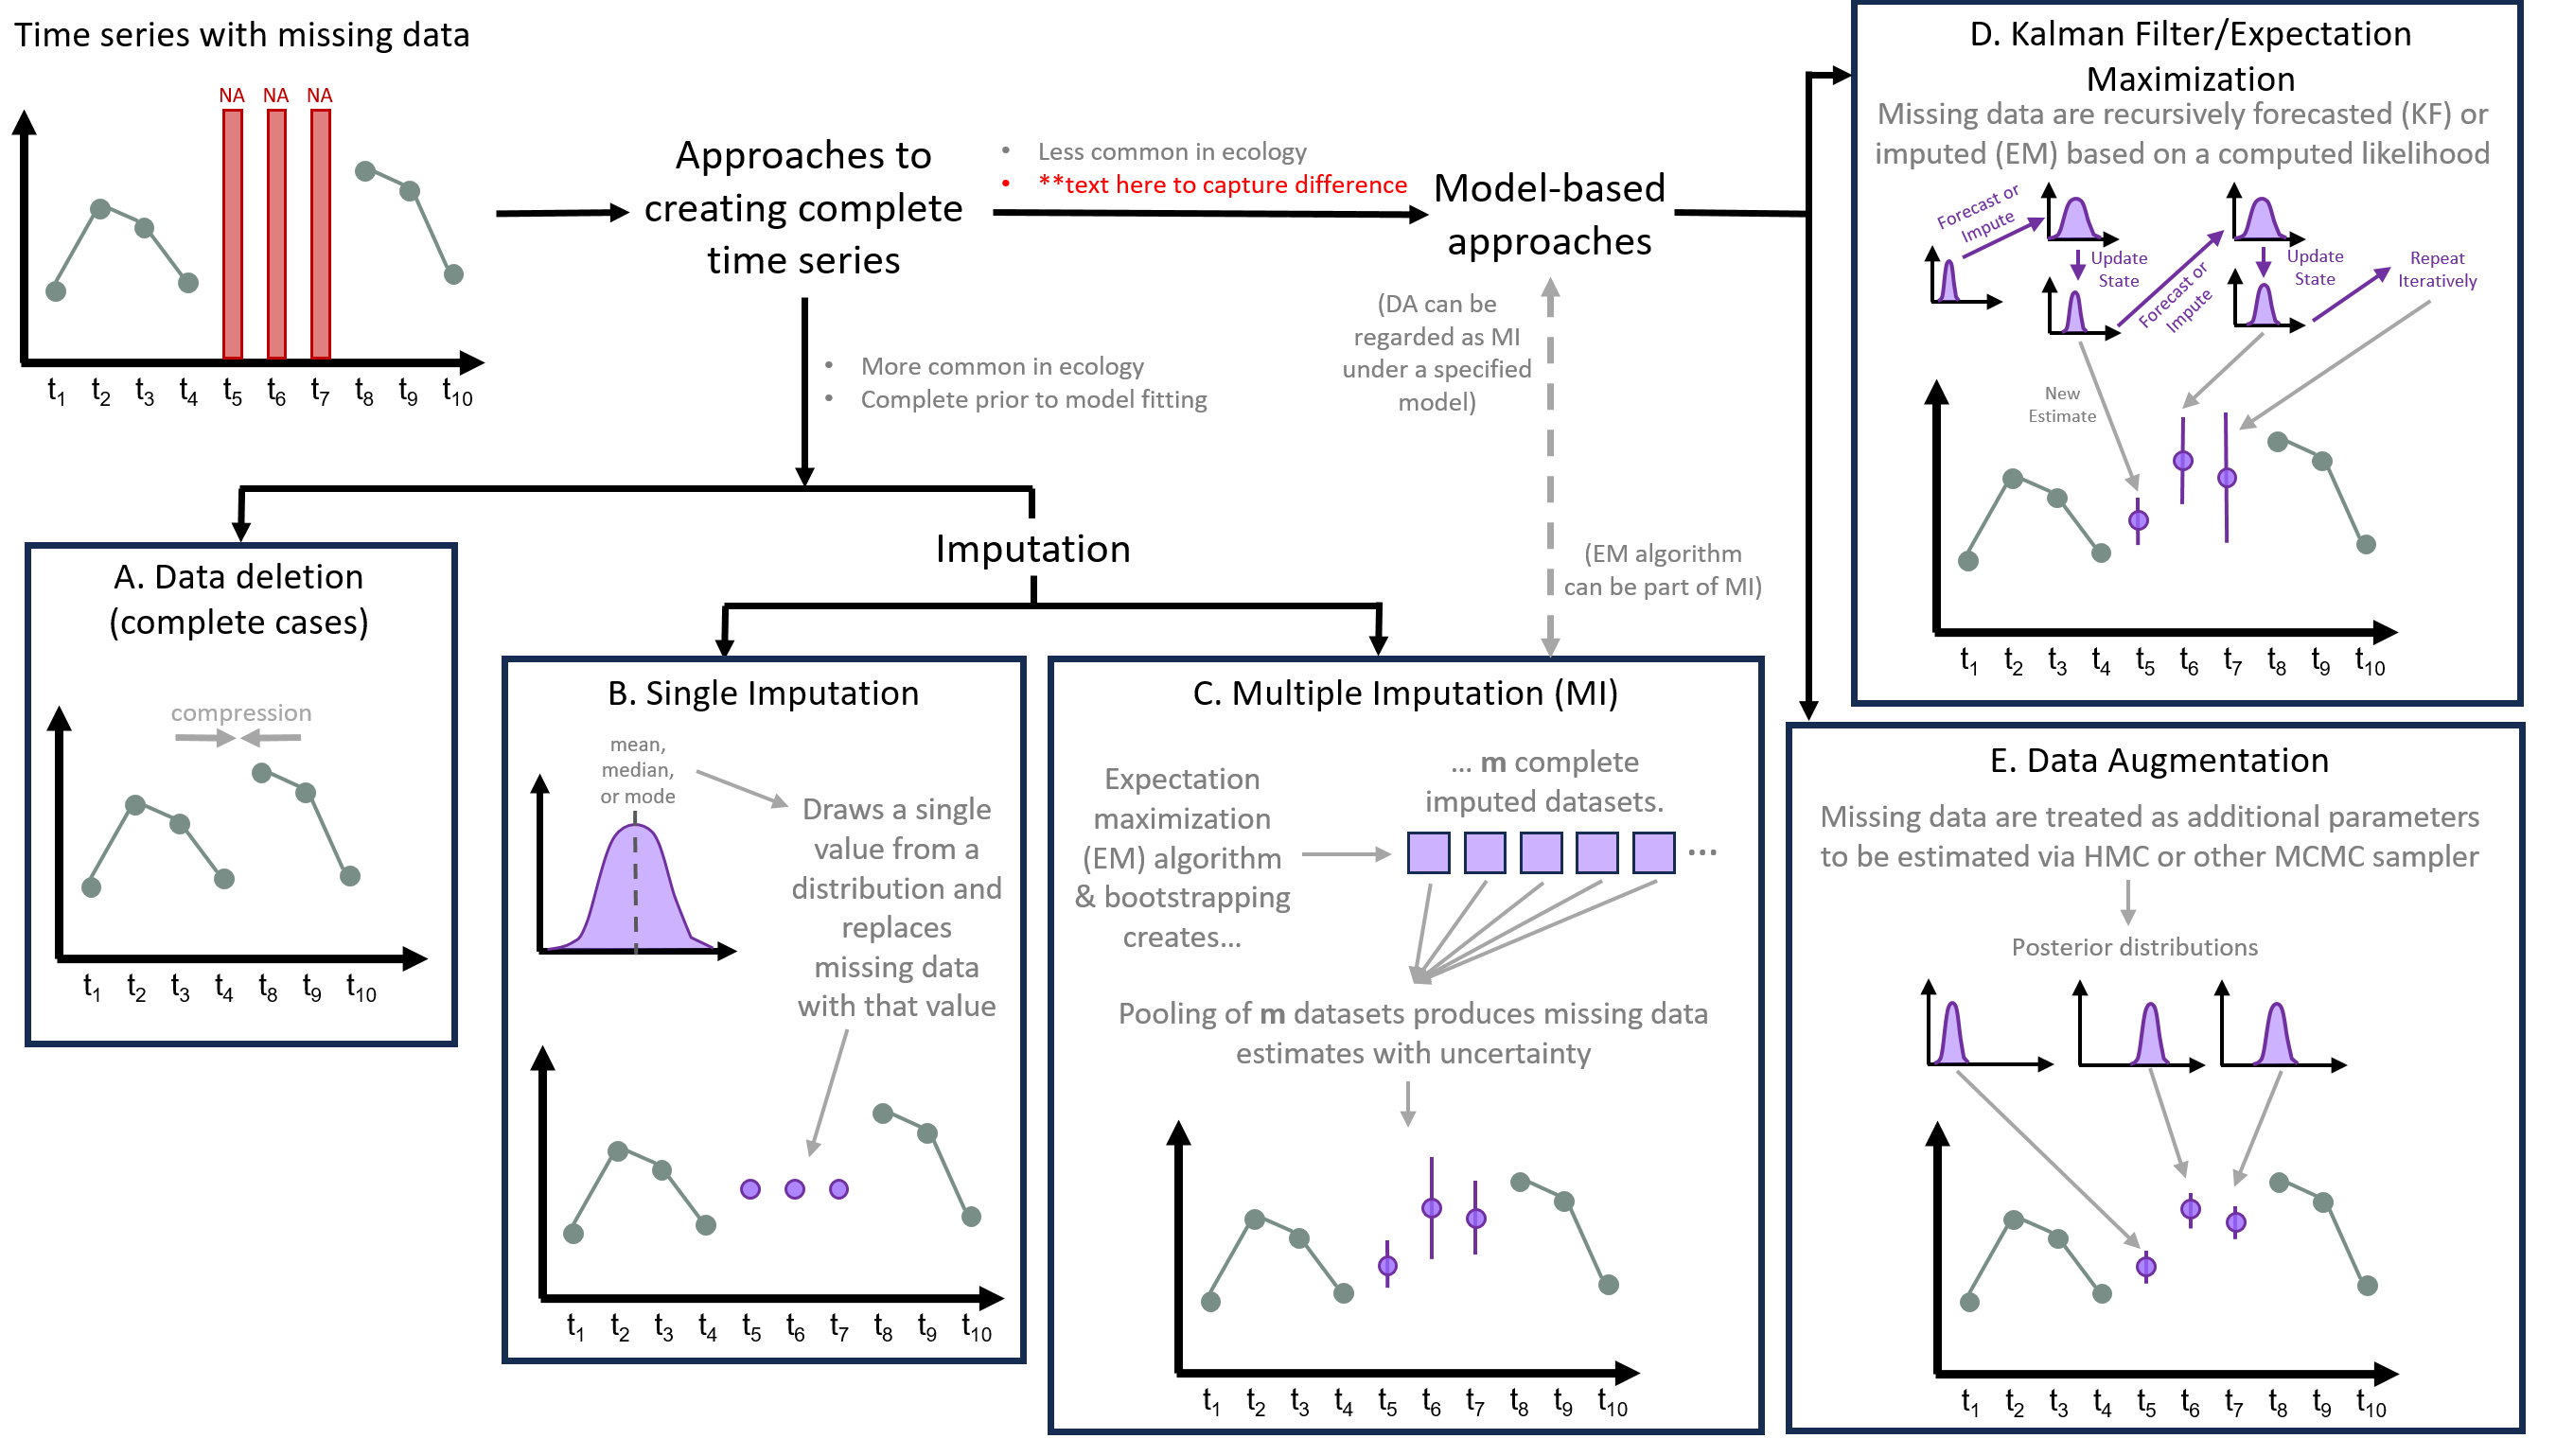
\includegraphics[width = 0.9\textwidth]{Figures/ConceptualFigure.png}
     \caption{Current (as of 1/8/24) draft of conceptual figure}
     \label{fig:ConceptualFigure}
 \end{figure}



\begin{figure}
    \noindent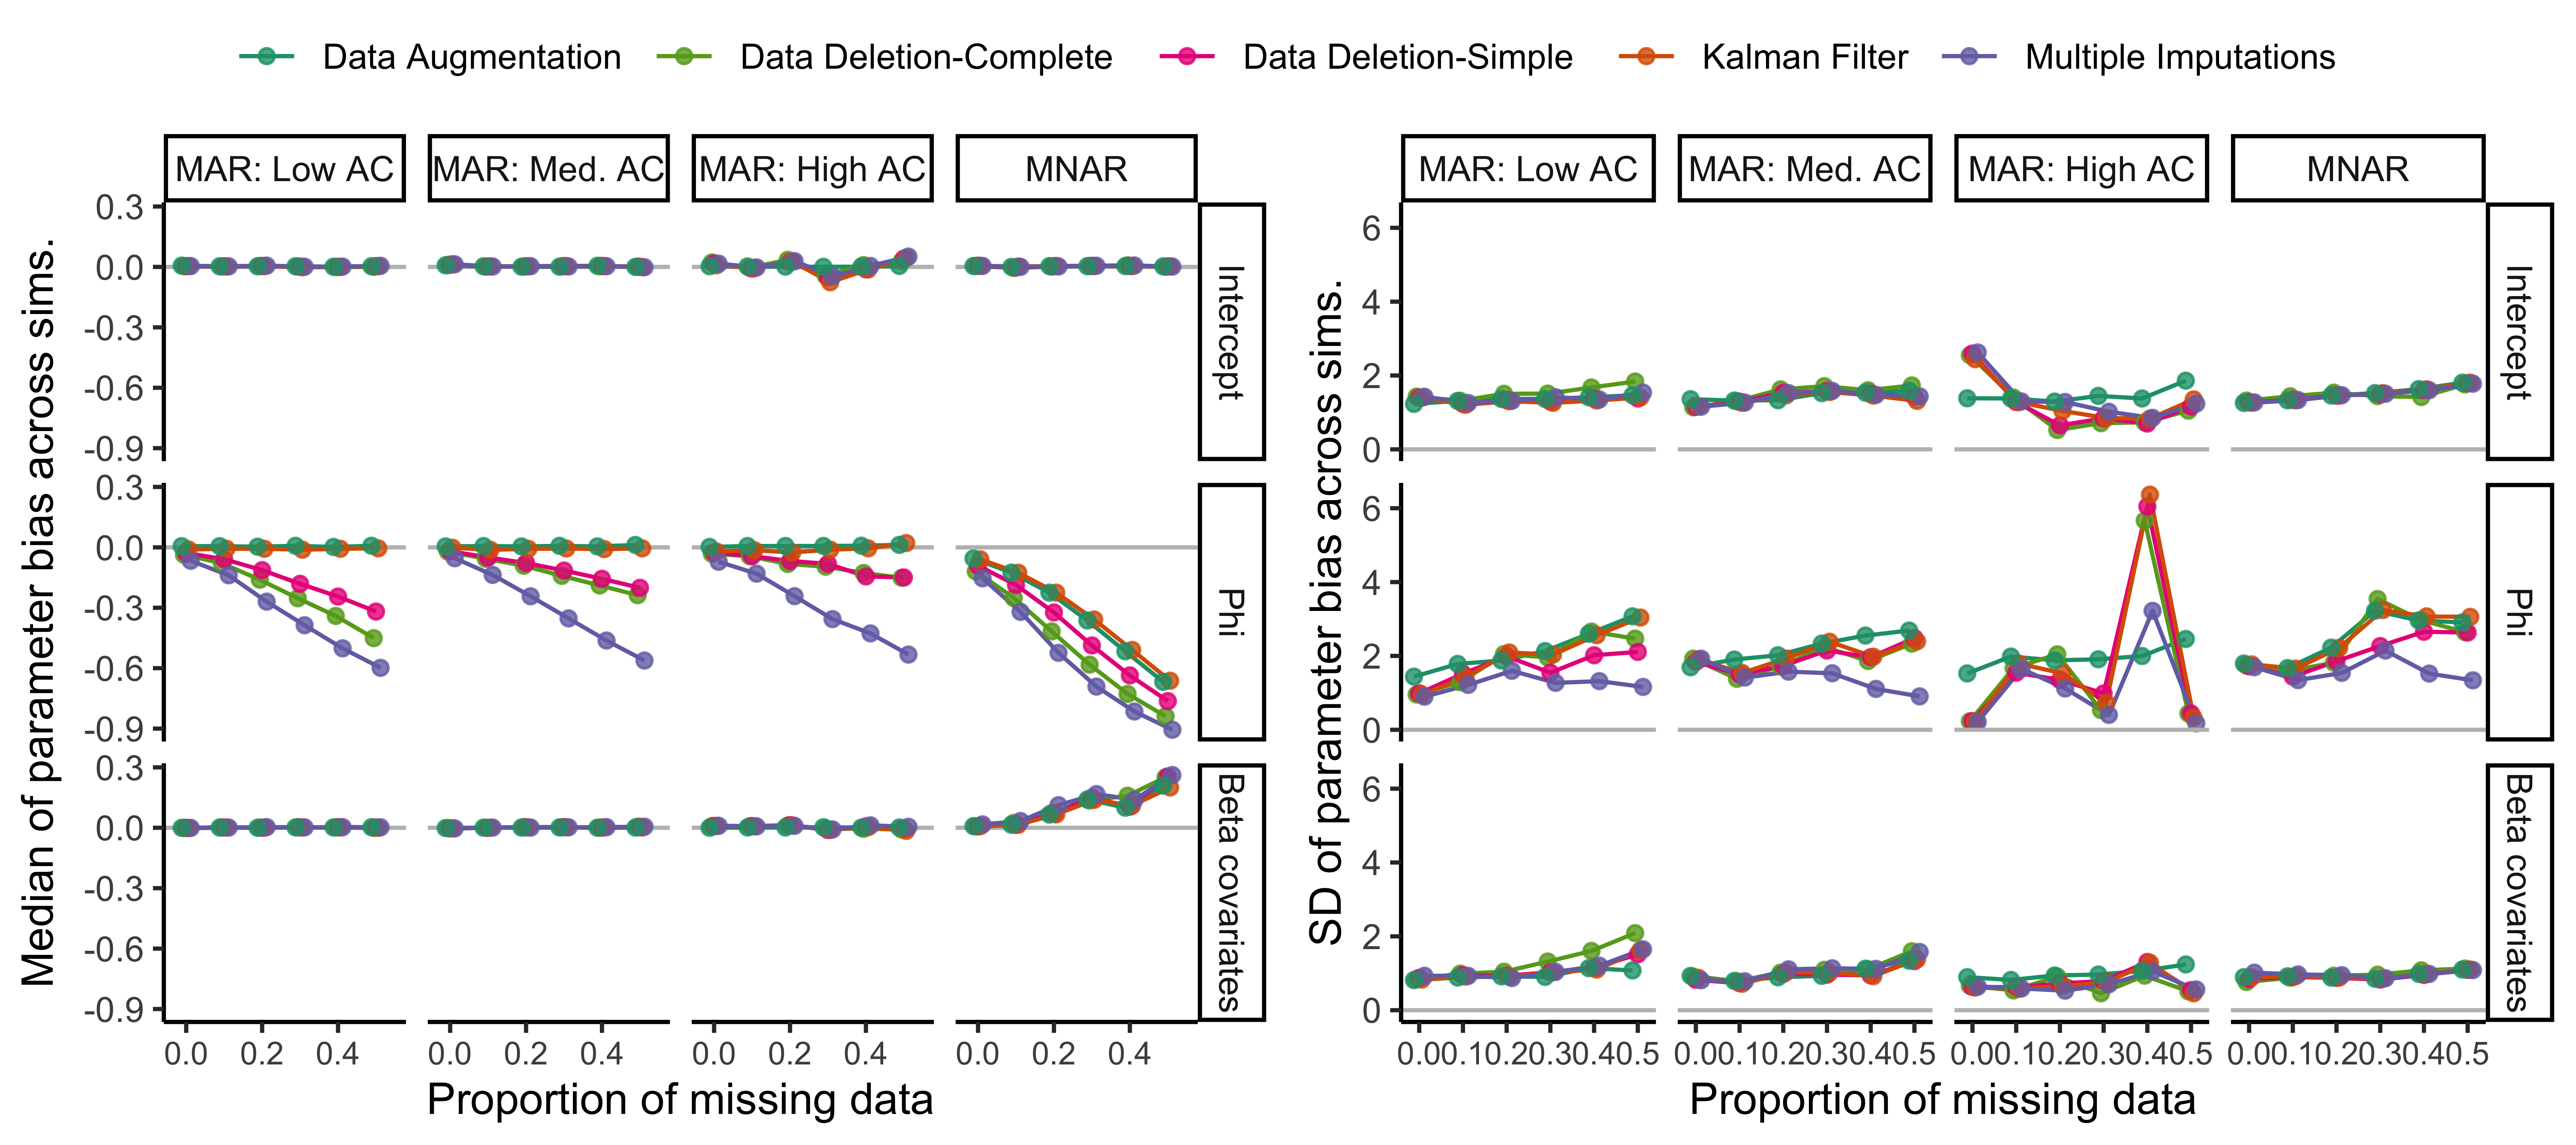
\includegraphics[width = \textwidth]{Figures/parameterRecovery_sim_Guassian_medsSD_trimmed.png}
    \caption{Medians and standard deviations of parameter estimate recovery using simulated Gaussian datasets--showing trimmed x-axis}
    \label{fig:ParamRec_Gauss}
\end{figure}

\begin{figure}
    \noindent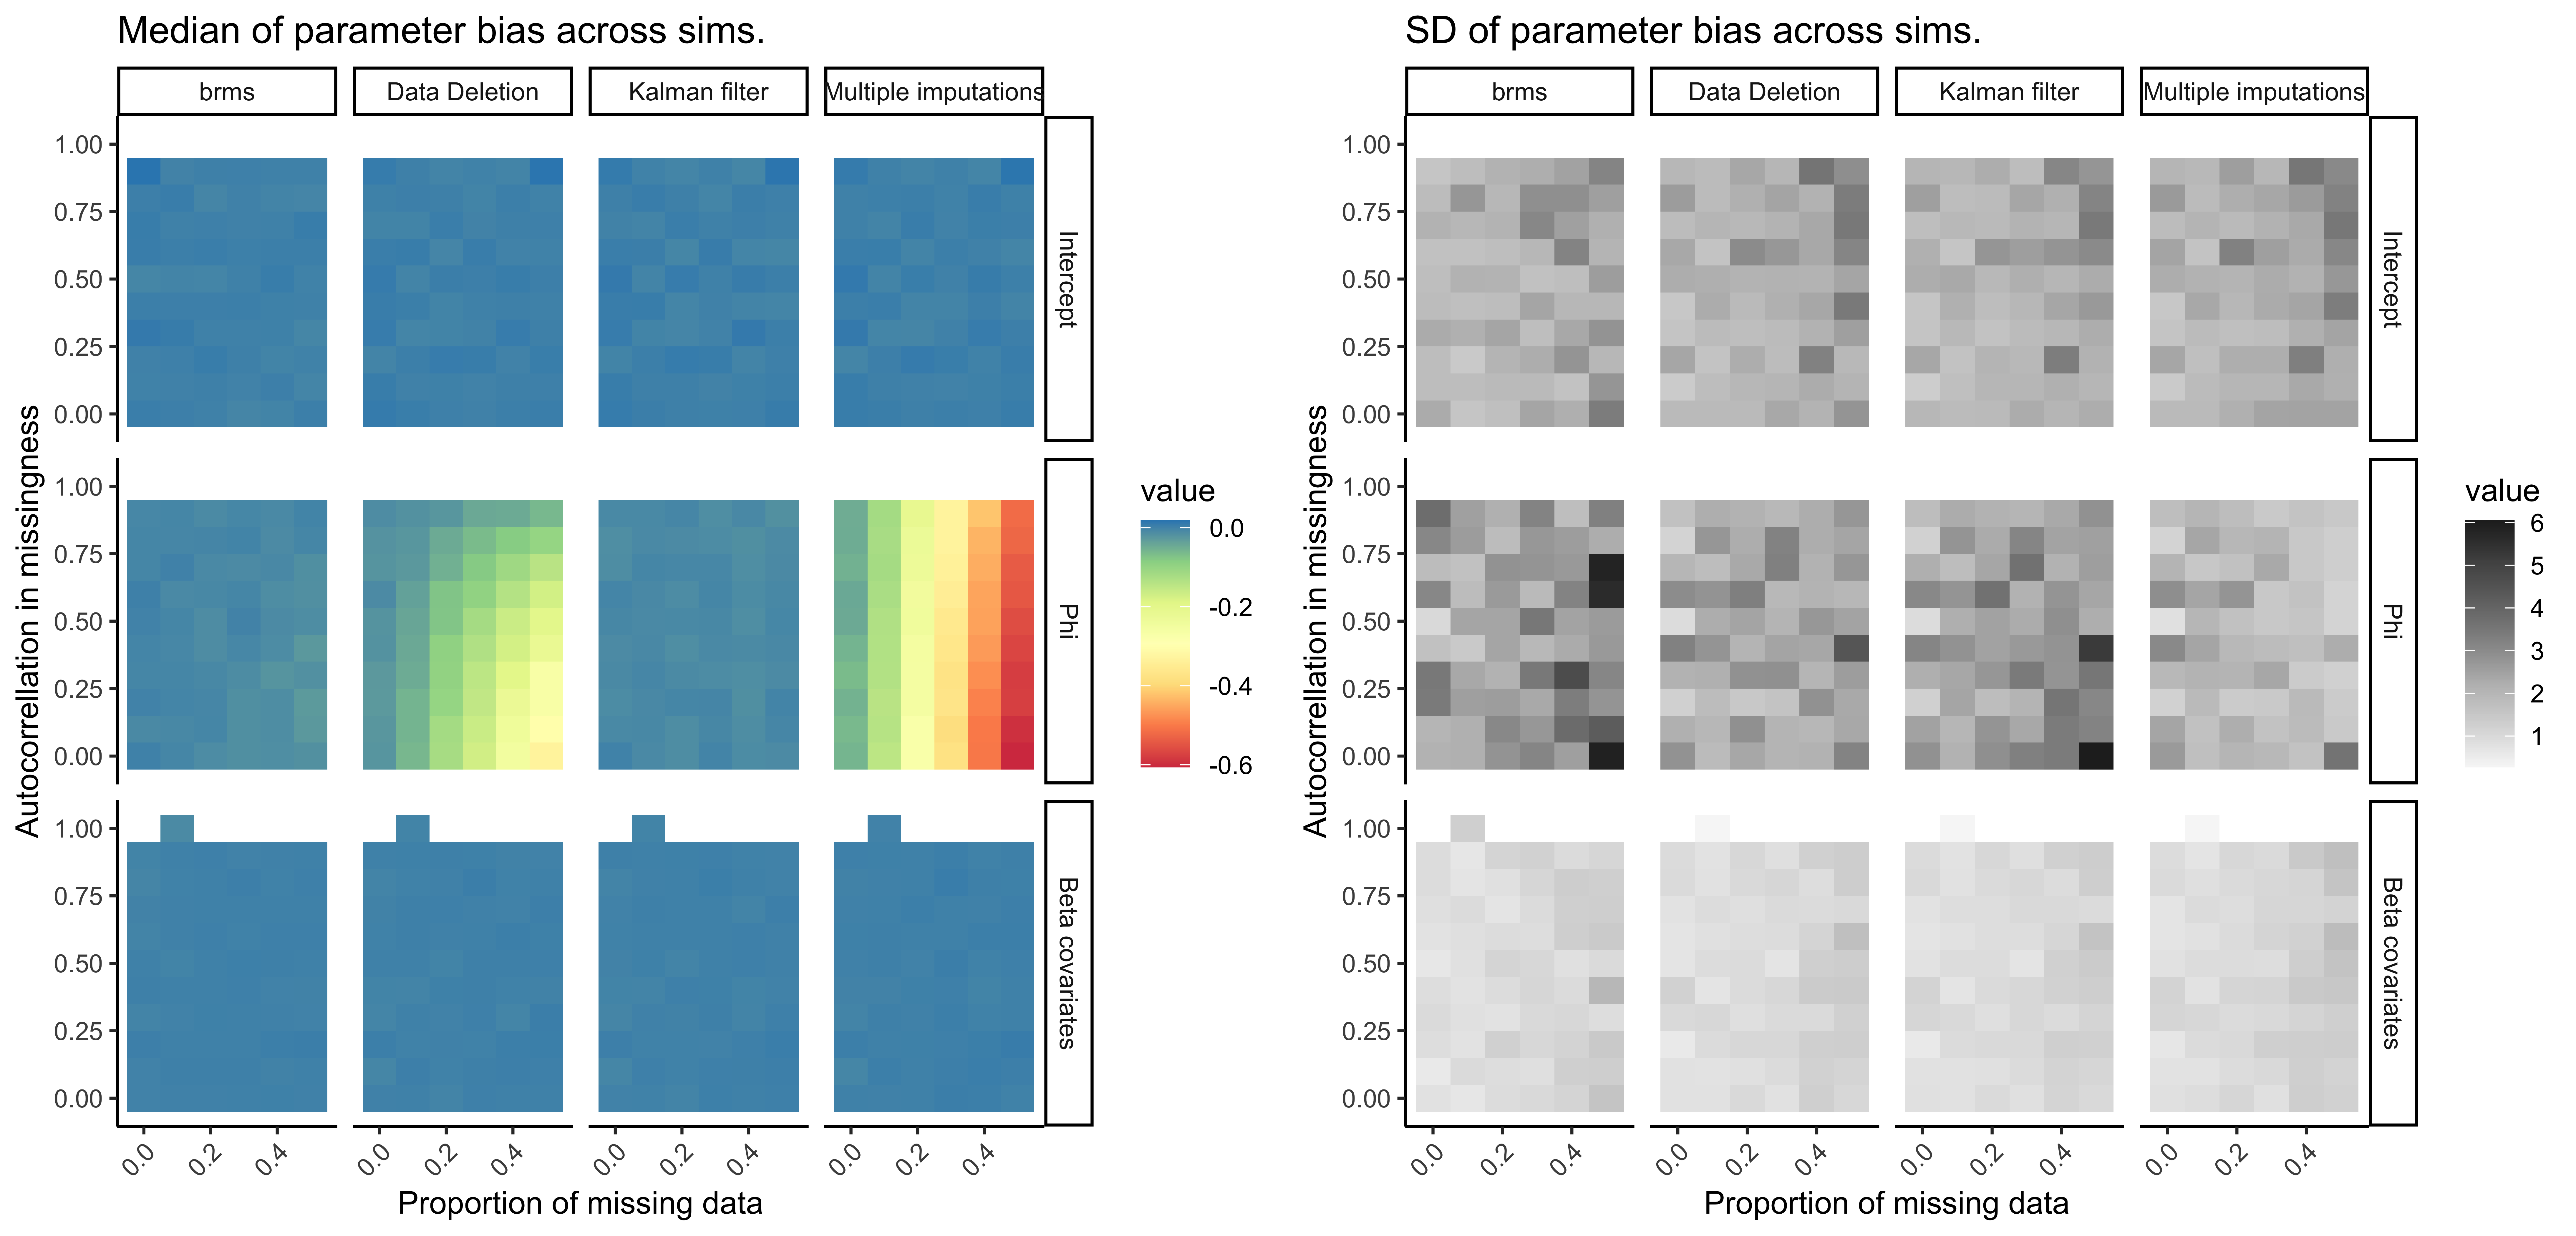
\includegraphics[width = \textwidth]{Figures/heatmap_GaussianMAR_all.png}
    \caption{Medians (A) and standard deviations (B) of parameter estimate recovery using simulated Gaussian datasets across all simulations w/MAR missingness. The grey horizontal line in A indicates the standardized true parameter value, and plotted values closer to this line indicate a more accurate model estimate of the true parameter.
    %AES make updates to these figures -- 1)remove grey line in SD panel, add panel letters (A and B) 2)change y axes in panel A? 3) make slightly wider to accomodate strip titles 4) change y-axis label to be less confusing
    }
    \label{fig:heatMap_gauss_MAR}
\end{figure}

\begin{figure}
    \noindent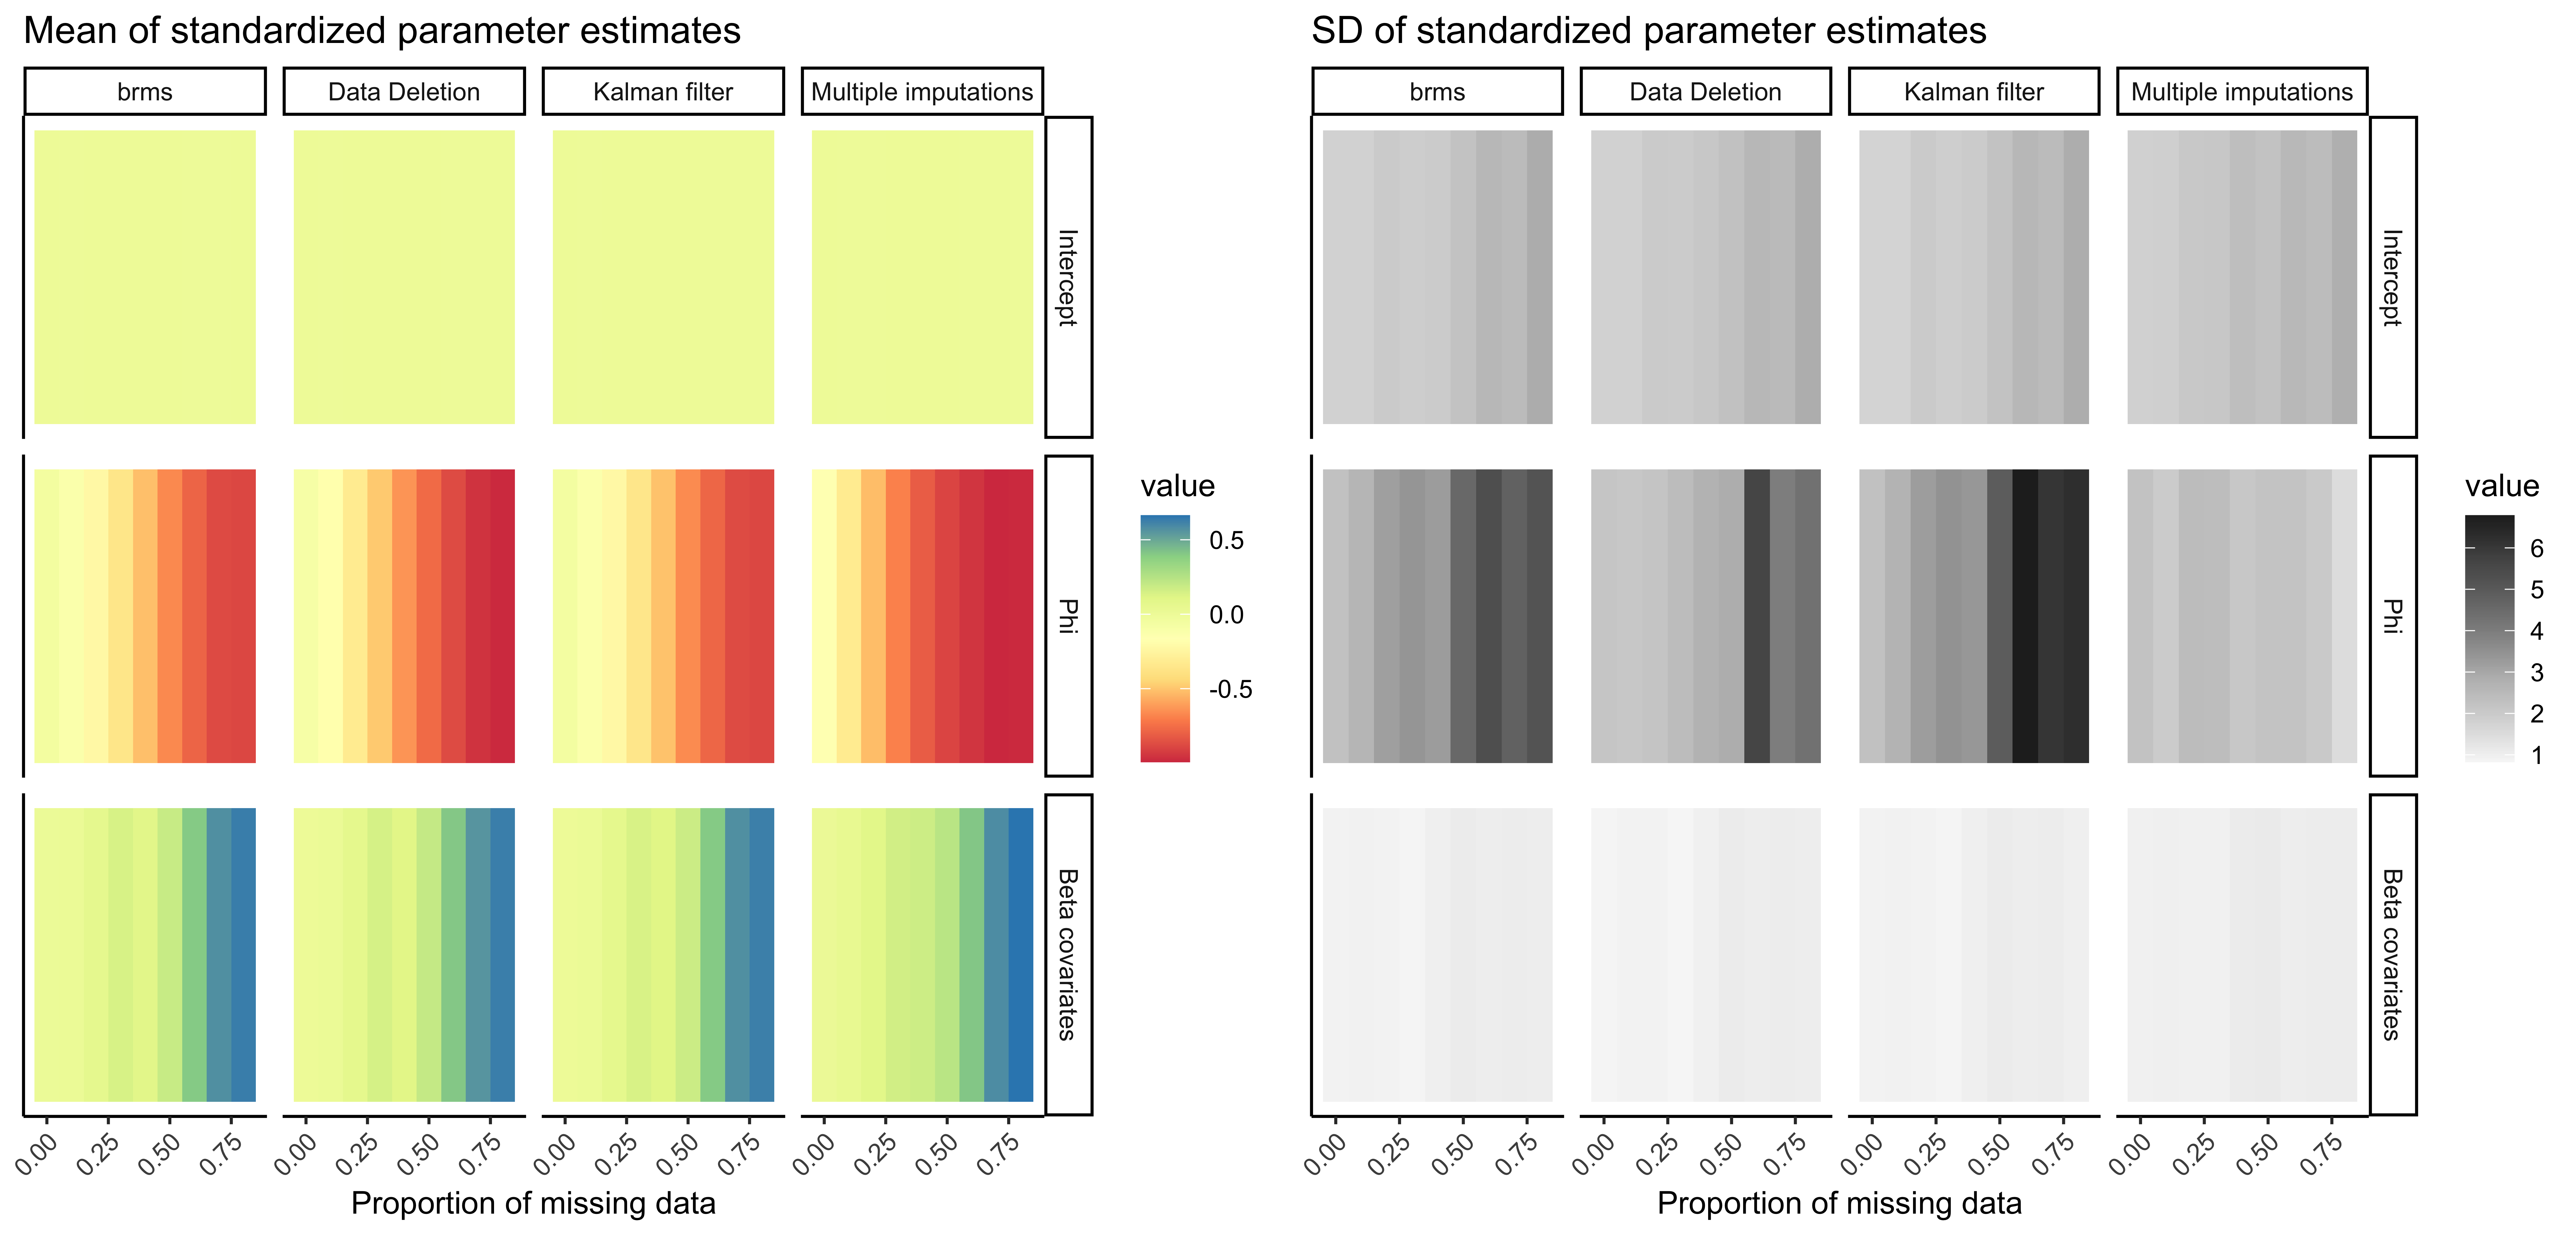
\includegraphics[width = \textwidth]{Figures/heatmap_GaussianMNAR_all.png}
    \caption{Medians and standard deviations of parameter estimate recovery using simulated Gaussian datasets across all simulations w/MNAR missingness (it says means,  but is actually medians, will change label)}
    \label{fig:heatMap_gauss_MNAR}
\end{figure}

\begin{figure}
    \noindent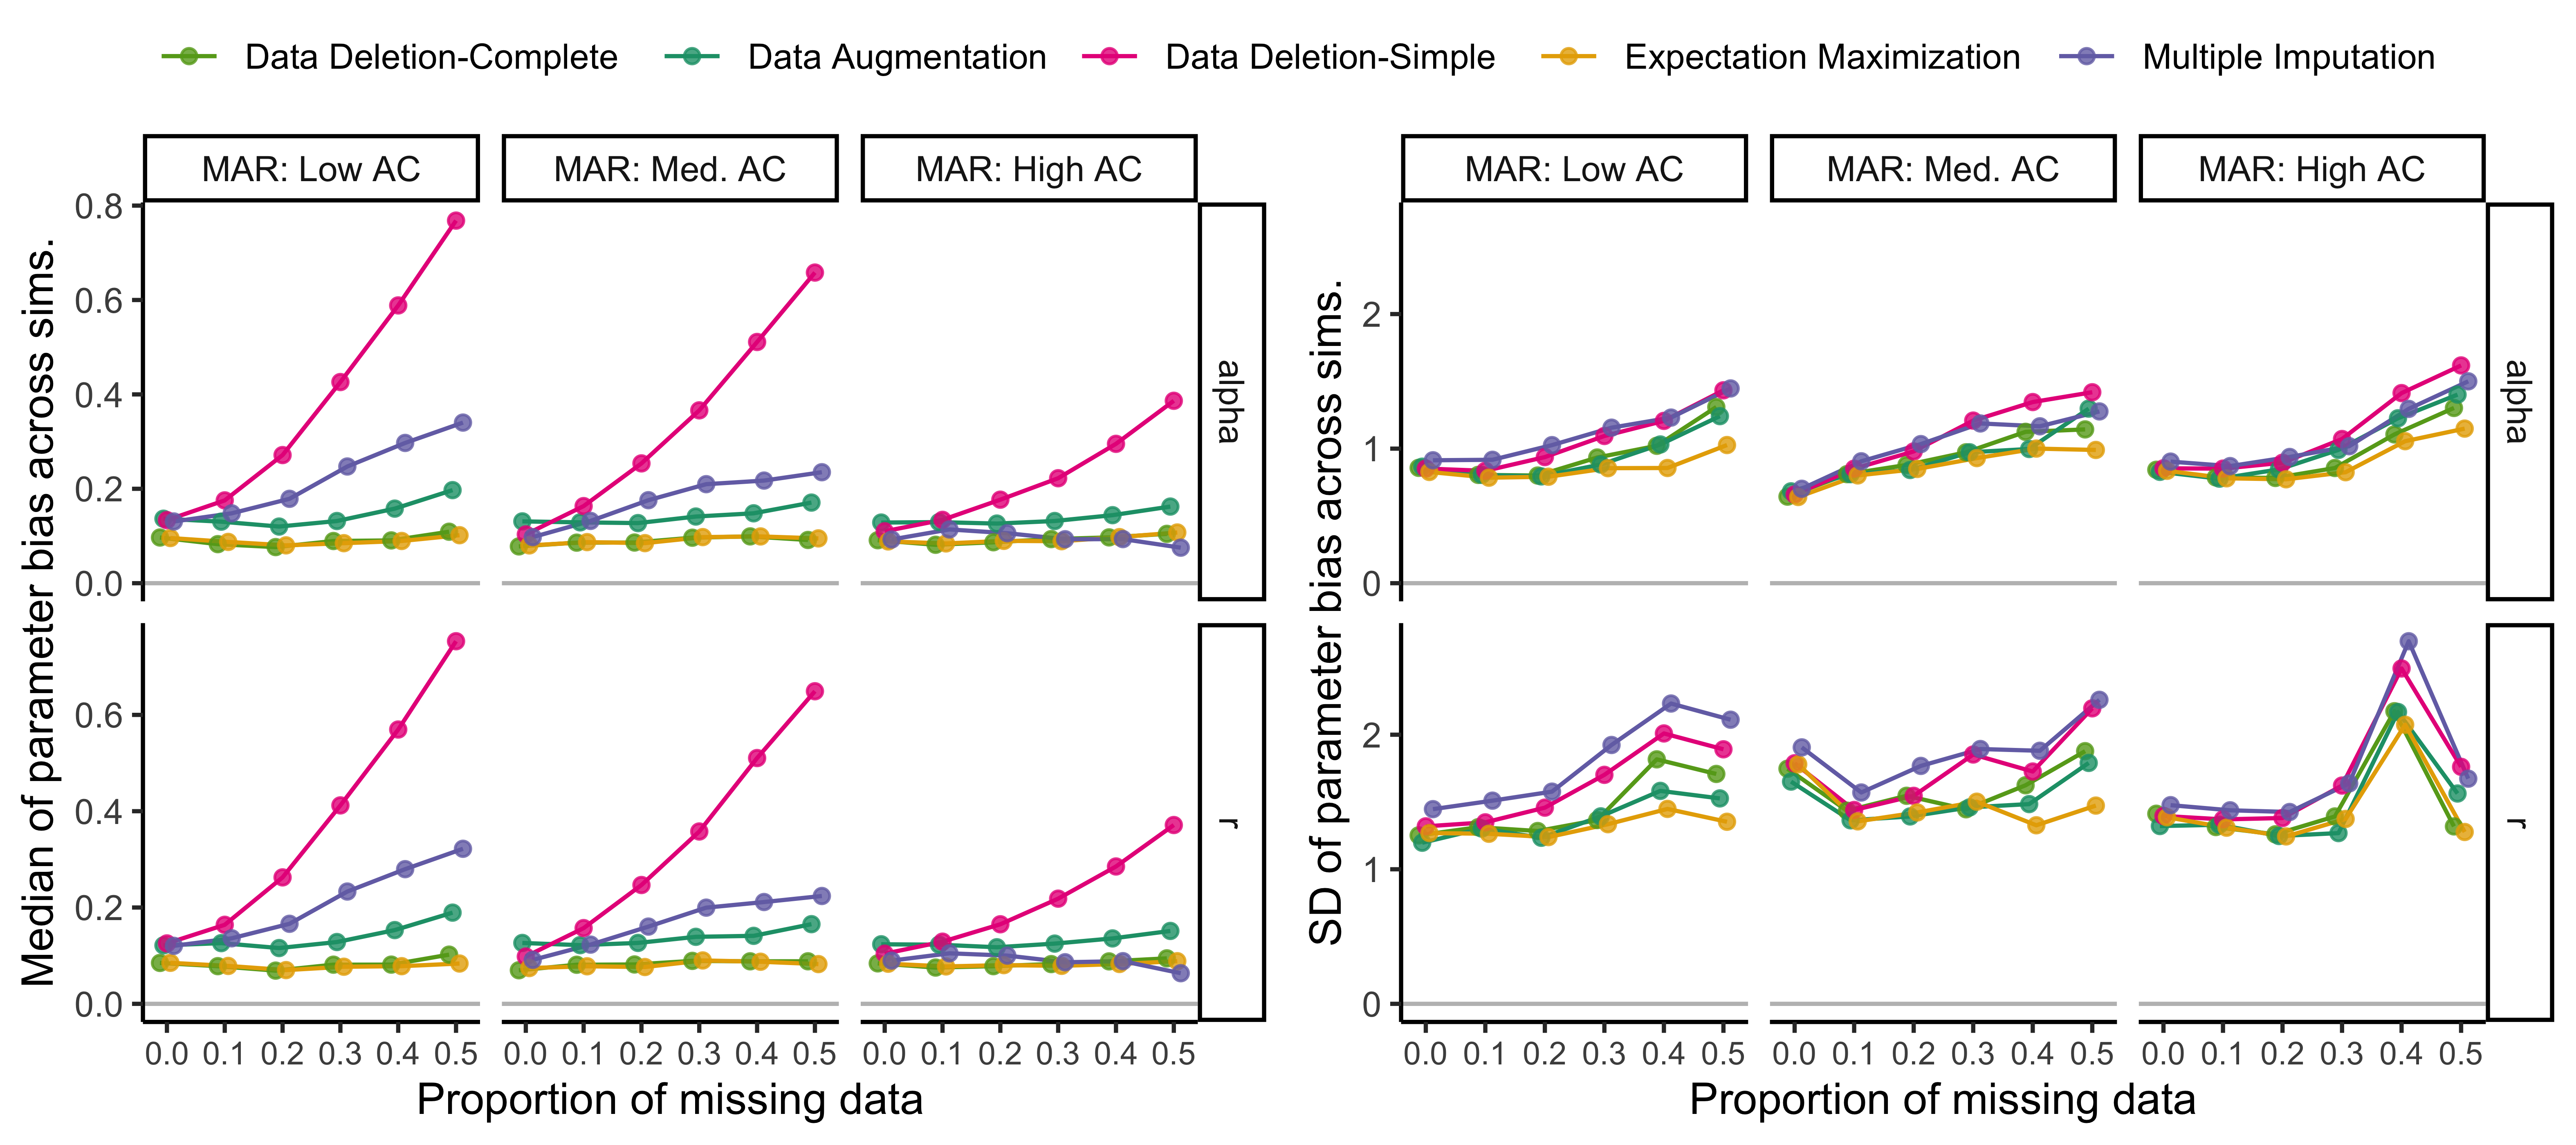
\includegraphics[width = \textwidth]{Figures/parameterRecovery_sim_Poisson_medsSD_trimmed.png}
    \caption{Medians and standard deviations of parameter estimate recovery using simulated Poisson datasets--showing trimmed x-axis}
    \label{fig:ParamRec_Poiss}
\end{figure}

\begin{figure}
    \noindent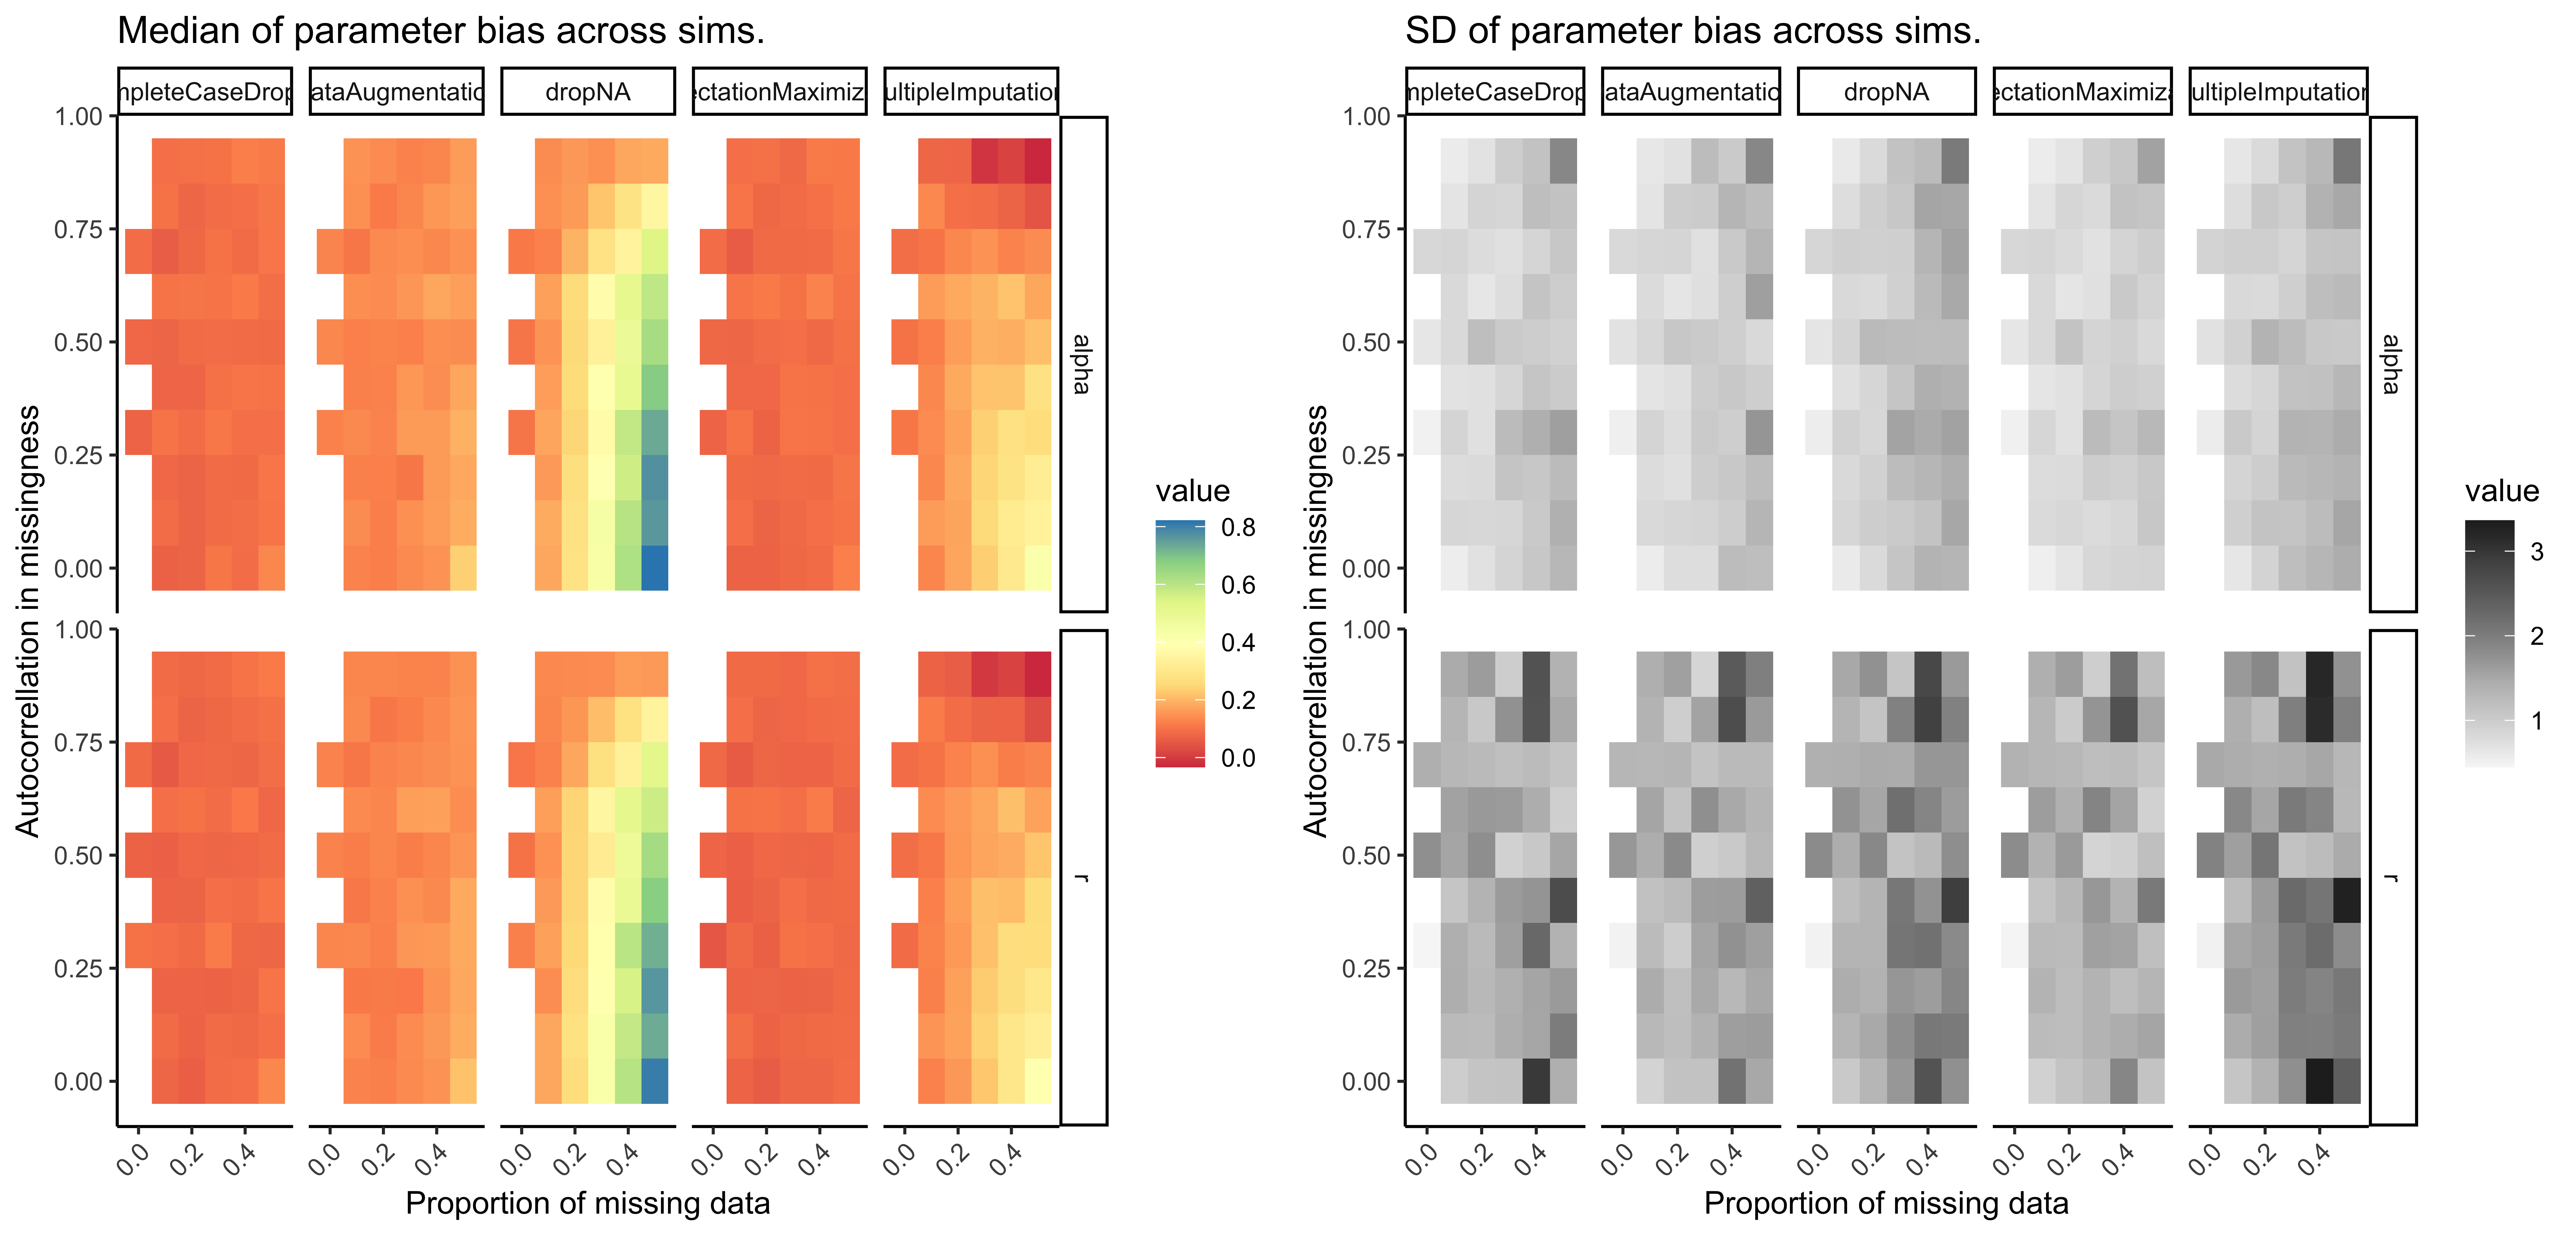
\includegraphics[width = \textwidth]{Figures/heatmap_PoissonMAR_all.png}
    \caption{Medians and standard deviations of parameter estimate recovery using simulated Poisson datasets across all simulations w/MAR missingness}
    \label{fig:heatMap_poiss_MAR}
\end{figure}

\begin{figure}
    \noindent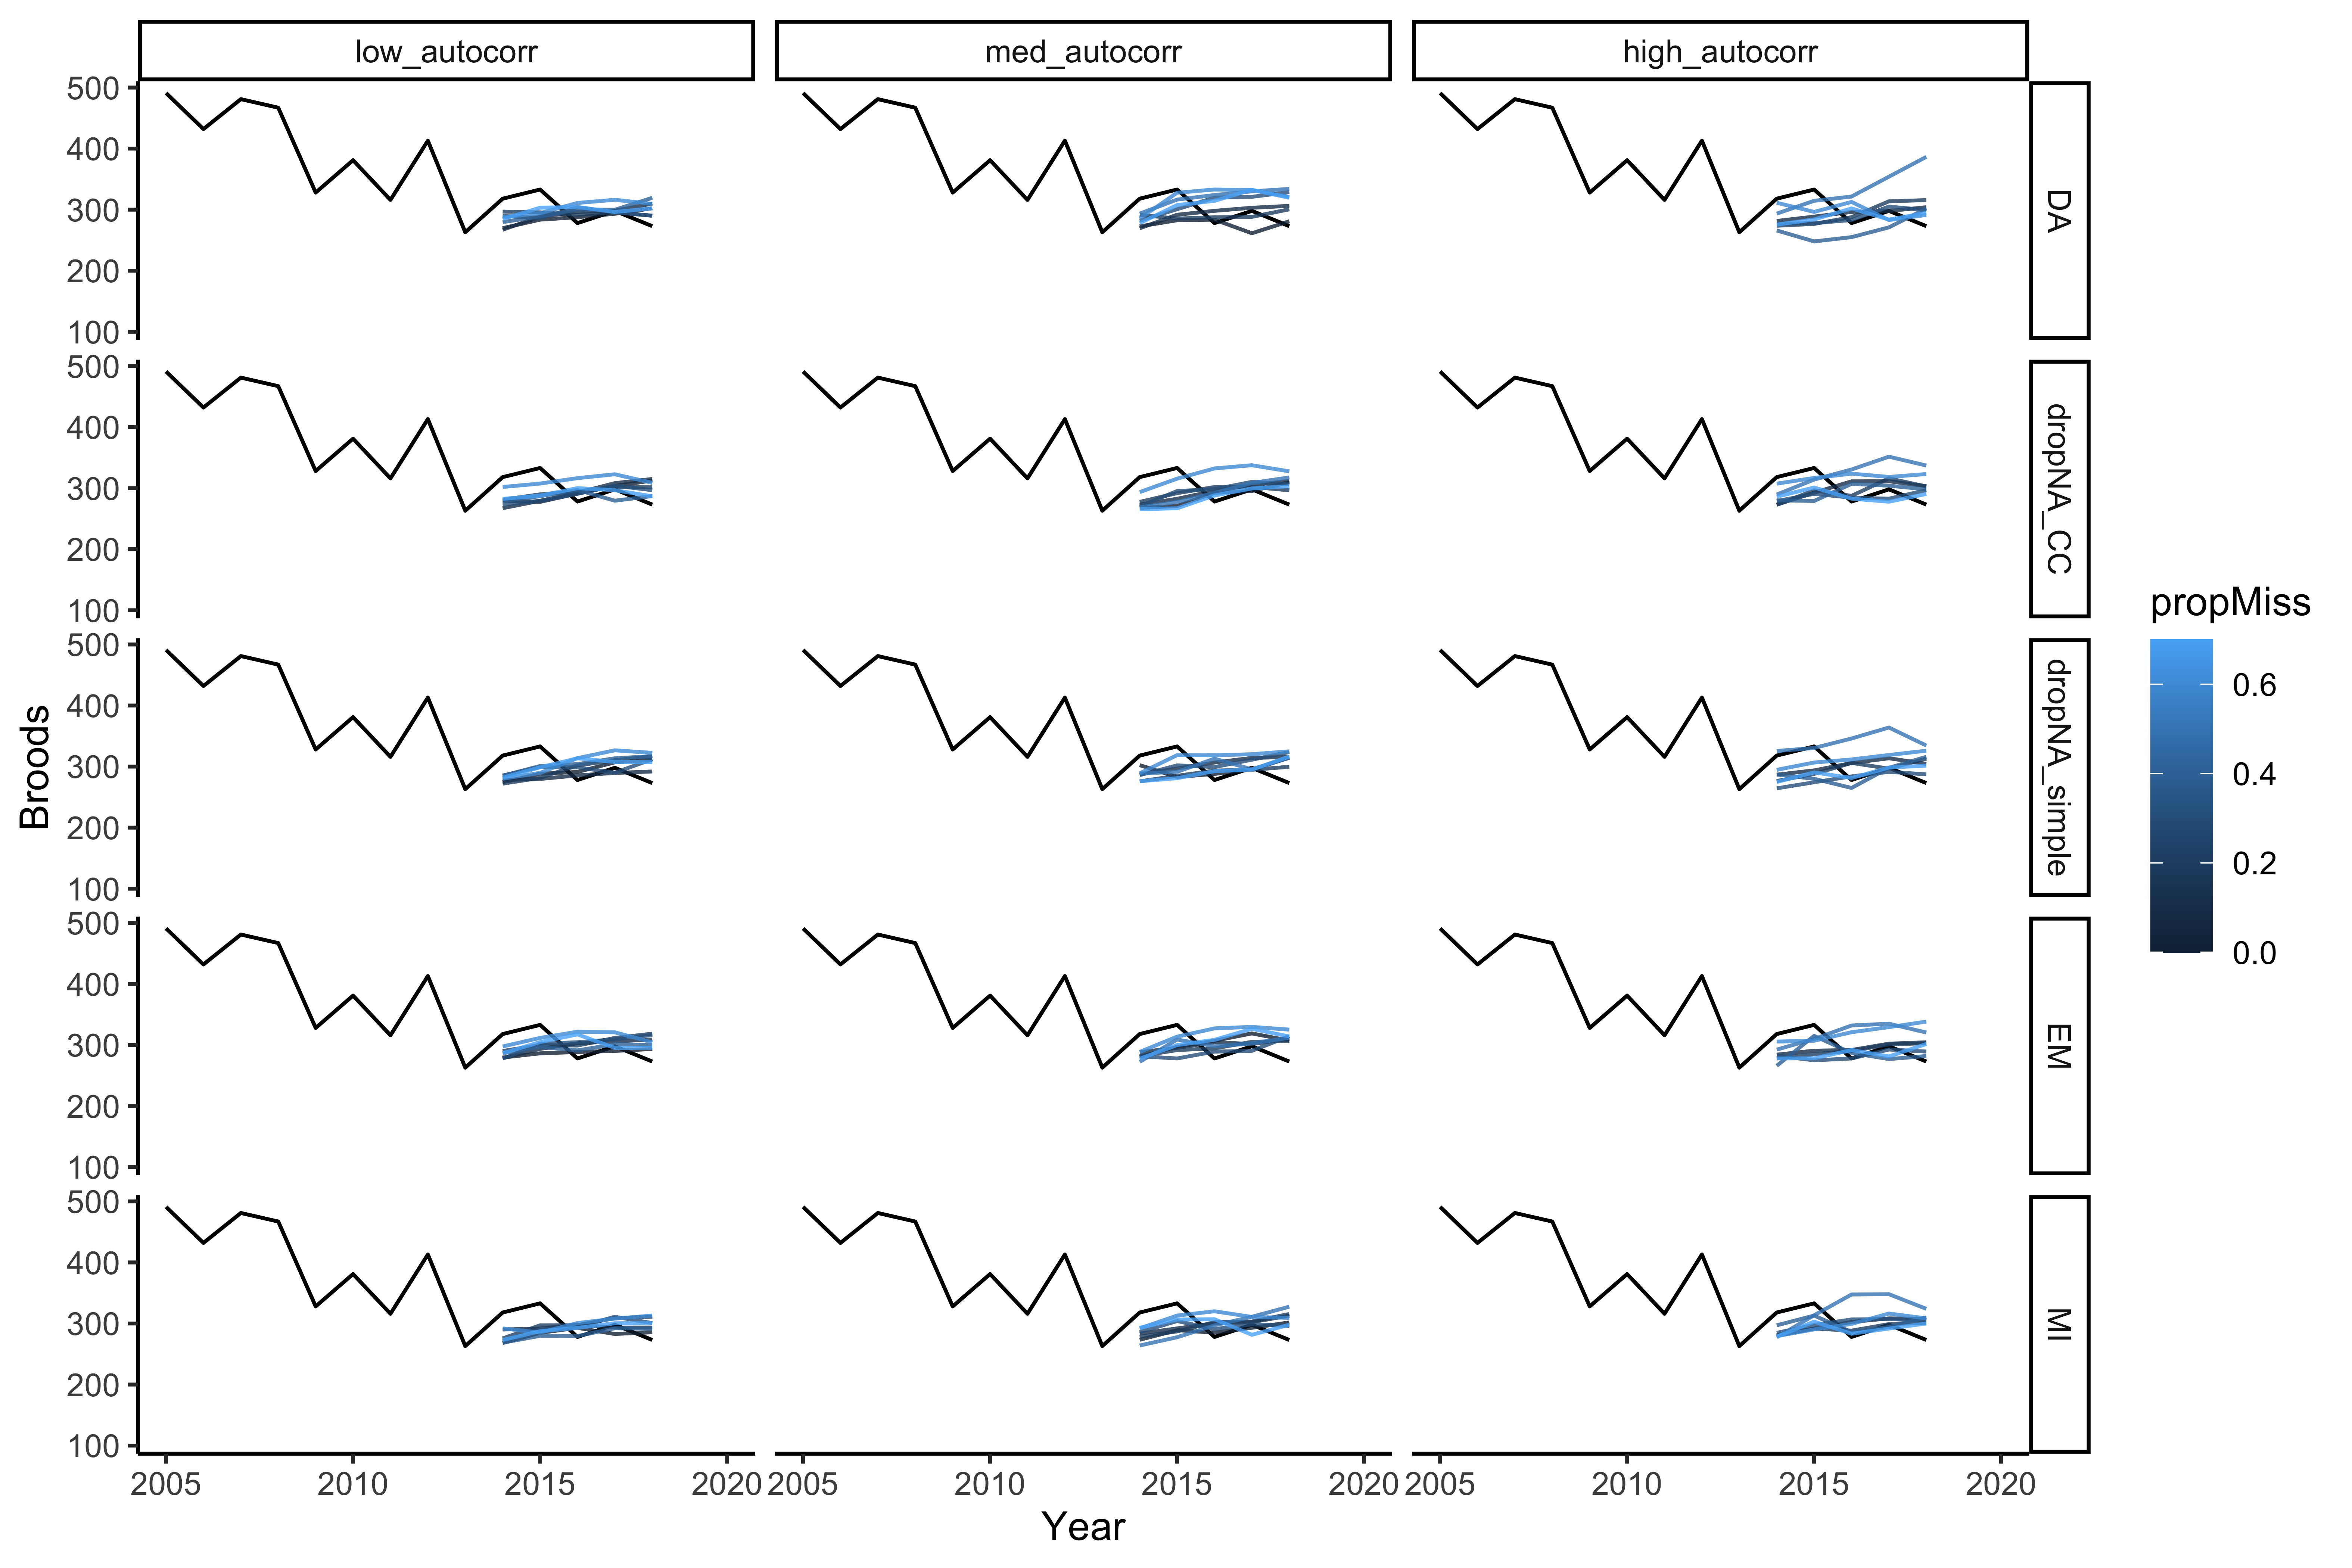
\includegraphics[width = \textwidth]{Figures/forecastAccuracy_poisson.png}
    \caption{Forecasted brood size (shown in shades of blue) from Ricker models fit to the Wytham Woods Great Tit dataset were generally similar to the true brood size (shown in black). Average forecasts are broken down by amount of autocorrelation (columns), missing data approach (rows), and amount of missingness (line color, ranging from dark blue for no missing data to light blue for 70\% missing data). Forecasts were generaly more accurate when autocorellation in missiness was low, but there were no other clear patterns in forecast accuracy. Note that the x-axis was truncated in this figure to show only the last 13 years of observational data. The Wytham Woods dataset consists of annual observations from 1960 through 2018.  }
    \label{fig:forecastAccuracy_poisson}
\end{figure}

\begin{figure}
    \noindent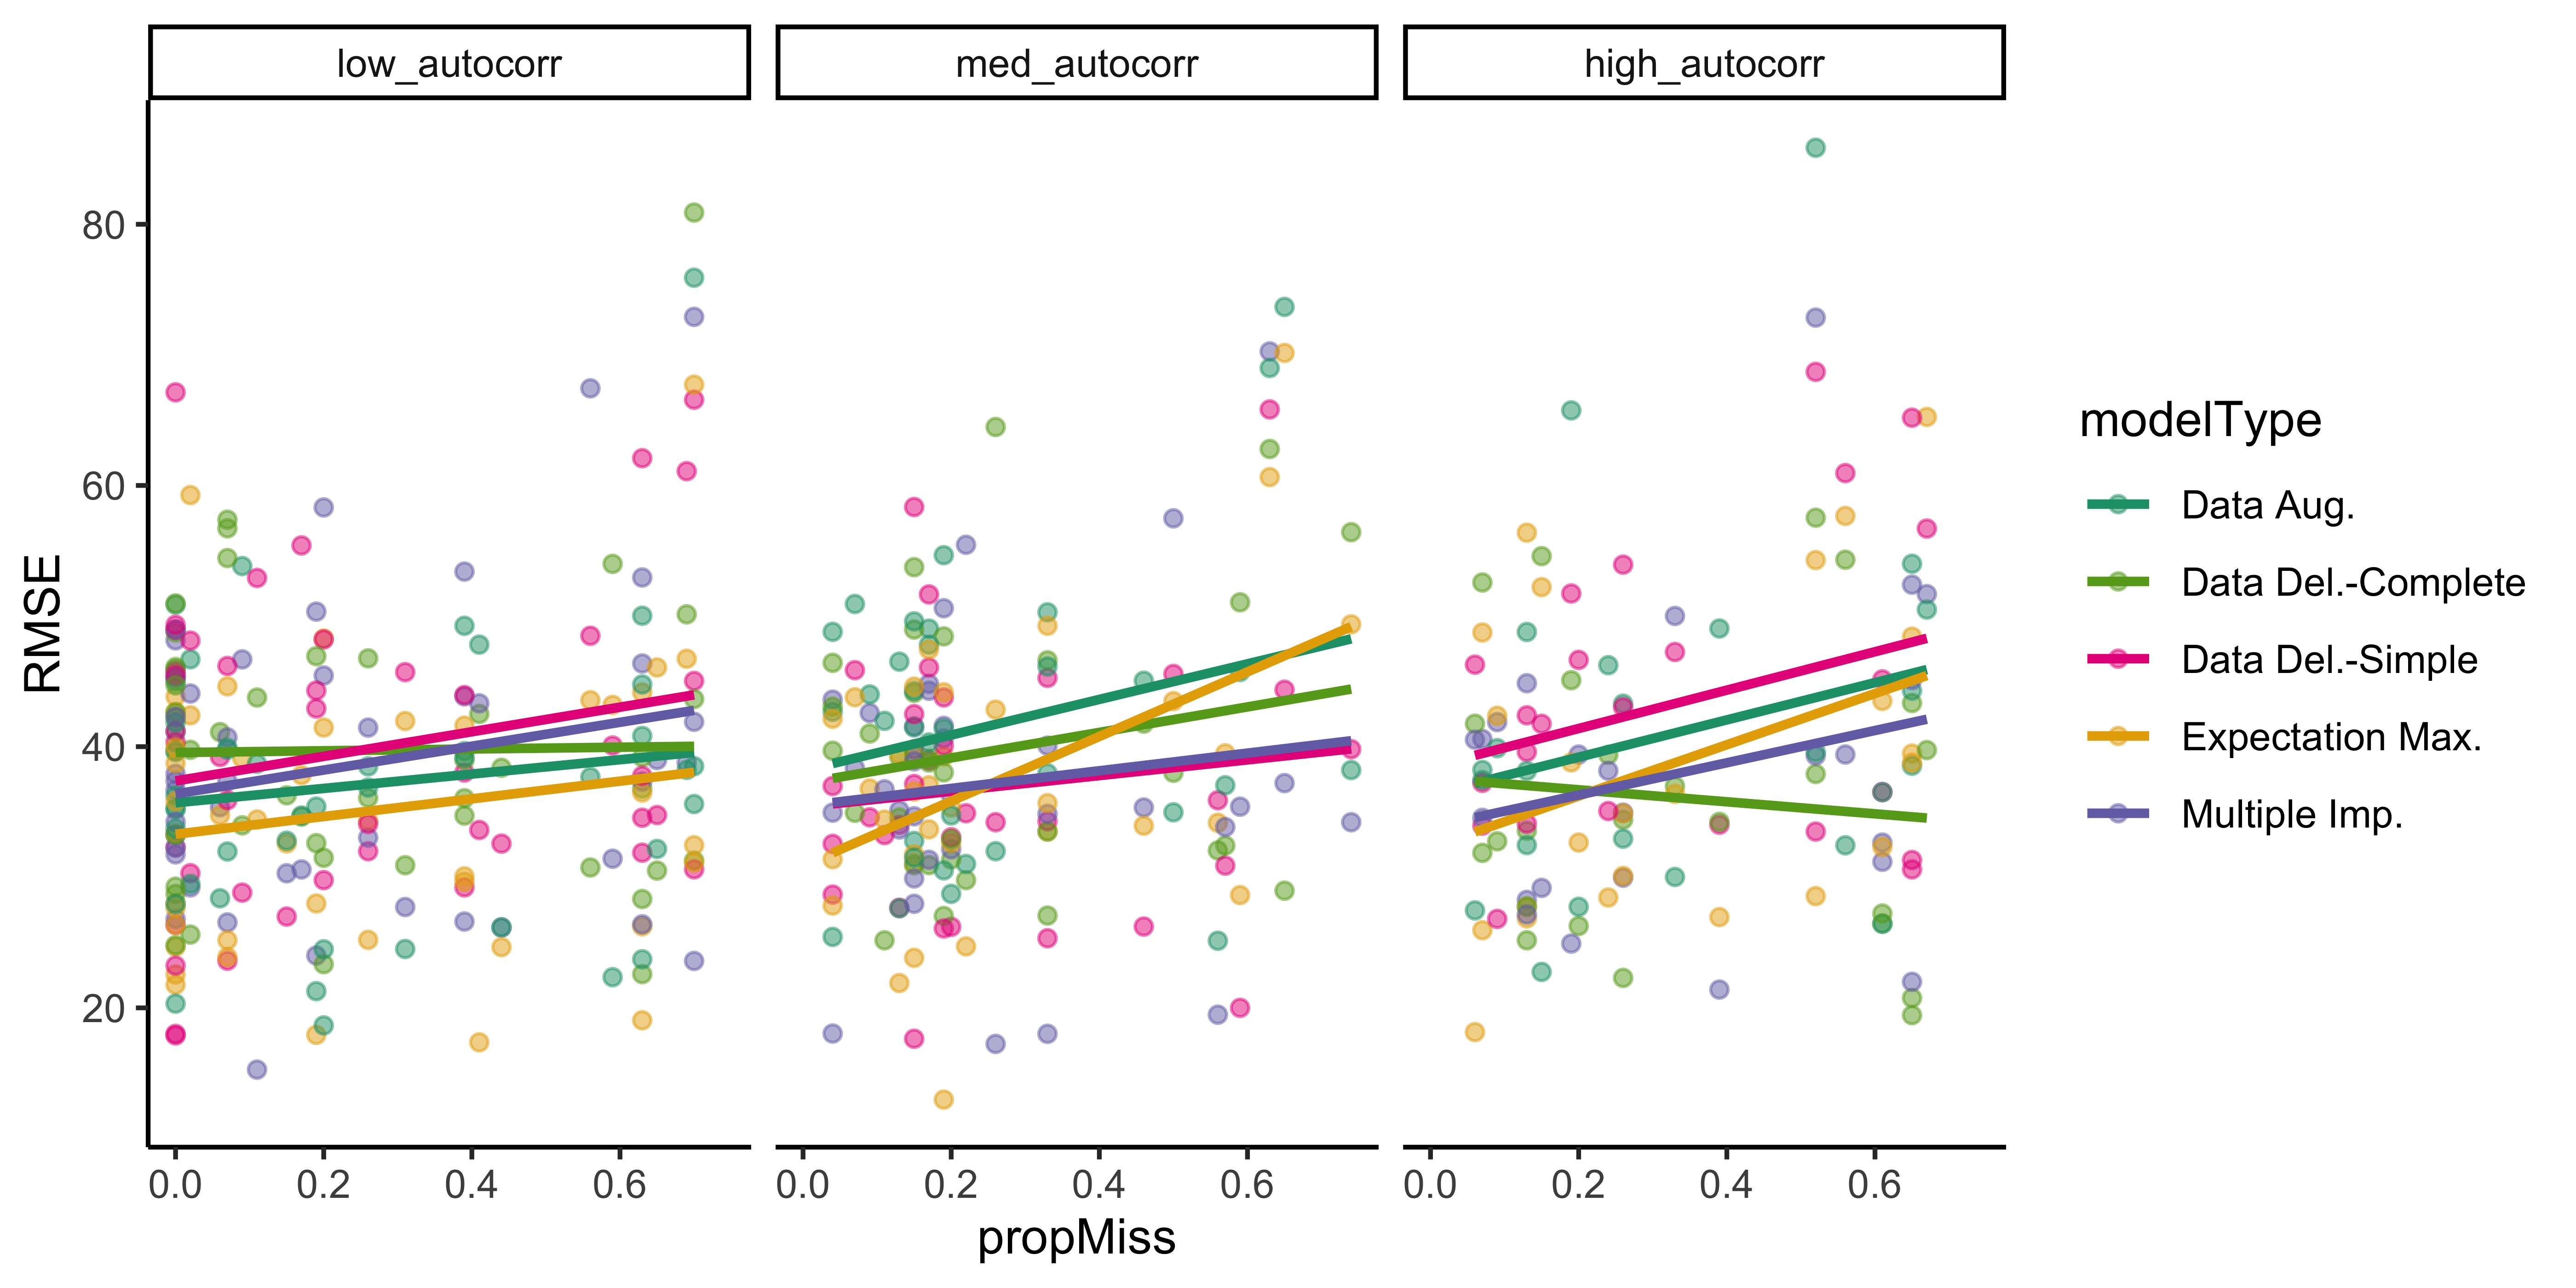
\includegraphics[width = \textwidth]{Figures/RMSE_poisson.png}
    \caption{In models using the Wytham Woods Great Tit Dataset with increasing levels of missingness, forecast RMSE generally increases as the amount of missingness increases. There are not clear differences between the average RMSE of models using different missingness approaches, nor is there a clear difference in patterns in model RMSE as the amount of autocorrelation changes.}
    \label{fig:forecastRMSE_poisson}
\end{figure}
\clearpage


\newpage

\bibliographystyle{ecology}
\bibliography{citations}

\newpage

%\appendix
\documentclass[12pt,english]{article} %12 pt for Ecology %
\usepackage[utf8]{inputenc}

\usepackage{geometry}                		
\geometry{verbose,letterpaper,tmargin=2.54cm,bmargin=2.54cm,lmargin=2.54cm,rmargin=2.54cm}   % 1 inch margins for Ecology   

\usepackage{multirow}
\usepackage{graphicx}		
\graphicspath{ {c:} }
\usepackage{setspace}
\usepackage[version=4]{mhchem}
\doublespace
\usepackage{siunitx}
\usepackage[
  backend=biber,
  style=apa,
  maxcitenames=2,
  natbib=true]{biblatex}
\addbibresource{citations.bib}
\usepackage{amsmath}
\usepackage{bm}
\usepackage{amsfonts}
\usepackage{lineno}
\usepackage{gensymb}
\usepackage[sharp]{easylist}%makes nice outlines.  Use # for symbol
\usepackage{blkarray}
\usepackage{lastpage}
\usepackage{times} % times new roman%
\usepackage{lineno} % add line numbers%

\begin{document}


\noindent\textbf{Journal}: Ecology; \textbf{Article Type}: Statistical Innovations

{\Large \noindent \bf %Approaches for handling missing data in ecological time series
Accounting for missing data in autoregressive models of ecological time series
}

%Journal name
%Manuscript type

\medskip

\noindent Alice E. Stears\textsuperscript{*, 1, 2}, 
Melissa DeSiervo\textsuperscript{*, 3, 2},
Dustin Gannon\textsuperscript{4, 2},
Amy Patterson\textsuperscript{5, 2},
Alice M. Carter\textsuperscript{6,7},
Joanna R. Blaszczak\textsuperscript{8},
Matt Trentman\textsuperscript{9},
Eliza Grames\textsuperscript{10},
Robert O. Hall, Jr\textsuperscript{7},
Joshua P. Jahner\textsuperscript{11, 2},
Saheed O. Jimoh\textsuperscript{2},
Courtenay A. Ray\textsuperscript{2},
Christa L. Torrens\textsuperscript{7},
Lauren Shoemaker$^{\circ}$\textsuperscript{2},
Christopher Weiss-Lehman$^{\circ}$\textsuperscript{2}

\noindent\noindent \textbf{Author affiliations}

\noindent\textsuperscript{1} Center for Adaptable Western Landscapes, Northern Arizona University, Flagstaff, AZ

\noindent\textsuperscript{2} Botany Department, University of Wyoming, Laramie, WY

\noindent\textsuperscript{3} Biology Department, Union College, Schenectady, NY

\noindent\textsuperscript{4} Department of Forest Ecosystems and Society, Oregon State University, Corvallis, OR 

\noindent\textsuperscript{5} Department of Biology, University of Maryland, College Park, MD

\noindent\textsuperscript{6} Department of Mathematics and Statistics, Utah State University, Logan, UT

\noindent\textsuperscript{7} Flathead Lake Biological Station, University of Montana, Polson, MT

\noindent\textsuperscript{8} Department of Natural Resources and Environmental Sciences, University of Nevada, Reno, Reno, NV

\noindent\textsuperscript{9} O’Connor Center for the Rocky Mountain West, University of Montana, Missoula, MT

\noindent\textsuperscript{10} Biological Sciences, Binghamton University, State University of New York, Binghamton, NY

\noindent\textsuperscript{11} Department of Biology, New Mexico Institute of Mining and Technology, Socorro, NM

\noindent\textsuperscript{*} Denotes equal contribution as lead author

\noindent{$^{\circ}$} Denotes equal contribution as primary investigator

\noindent \textbf{Corresponding author}: Alice Stears, alice.e.stears@gmail.com 


\section*{Appendix S1}


\subsection*{Introducing Missingness}

We created MCAR datasets with varying proportions of missing data and degrees of autocorrelation in missingness (Fig. \ref{fig:missingtypes} B--E) by viewing a time series as a Markov-modulated Bernoulli process where the variable could have two states: missing or not missing \citep{Gharib2014, Edwards1960}. The probability that an observation in a time series at time $t+1$ was missing depended on both the specified proportion of non-missing values in the entire time series ($p$) and the specified degree of autocorrelation in missingness ($\omega$). In a time series $X_1, X_2, ..., X_n$, the transition matrix that describes the probability of an observation at $X_{t+1}$ being missing, based on whether the observation at $X_t$ was missing is defined as: 


\begin{equation}
\begin{blockarray}{rcccc}
\text{} & \BAmulticolumn{4}{c}{X_{t+1}}\\
X_t & \text{Present} & \text{Missing}  \\
\begin{block}{r(cccc)}
\text{Present} & 1-(1-\omega)p & (1-\omega)p \\
\text{Missing} & (1-\omega)(1-p) & \omega + (1-\omega)p  \\
[1ex]
\end{block}
\end{blockarray}
\end{equation}


We created MNAR datasets with various proportions of msising data by first calculating the mean and standard deviation of the time series with no missing data, then using these point estimates as the mean and standard deviation of a normal distribution. We then identified the quantiles of that normal distribution above and below which the density of the normal distribution corresponded to the desired proportion of missingness. We replaced any values above and below those quantiles with an NA.

\subsection*{Missing Data Approaches} 
\textbf{Simple and Complete Data Deletion}: The ``simple data deletion" approach involves removing missing values from a time series, compressing the dataset, and running the model as if the time intervals between observations were all equal (Fig. 1 A). This method violates the assumption of equal temporal spacing between observations, an assumption implicit in most time series models. We include it here as a reference because it is simple and commonly used in published studies. We also include ``complete case data deletion," which maintains equal spacing between observations by removing a missing value itself as well as the subsequent observation(s) that is predicted by the missing value (Fig. 1 A). However, those observations after a missing value are retained as predictors of the subsequent observation(s). 

\textbf{Multiple Imputation}: Multiple imputation (MI) is an approach that systematically fills in missing observations with imputed values, and creates several versions of complete data sets that can be used to estimate uncertainty around each imputed value (Fig. 1 B). MI is commonly used in ecology, with multiple studies evaluating methods and approaches to conduct MI for functional traits \citep{taugourdeau_filling_2014,johnson_handling_2021,penone_imputation_2014}, population biology \citep{onkelinx_working_2017}, time series \citep{hui_gap-filling_2004}, and meta-analyses \citep{ellington_using_2015}. Multiple Imputation’s (MI) effectiveness can depend on the number of imputed datasets (\textit{m}). It is often assumed that \textit{m}=5 is a minimum value \citep{honaker_what_2010}; however, researchers have used \textit{m}=200 when comparing methods in the ecological sciences \citep{onkelinx_working_2017}. In general, larger values of \textit{m} result in more accurate estimates of both parameter values and uncertainty. However, increasing \textit{m} results in a trade-off between accuracy and computation time; this can be particularly problematic for data-rich (e.g., long time series) or complex (e.g., hierarchical) models. 
After imputing the \textit{m} data sets, the analyses of interest are confronted with each data set, and the estimated parameters from the \textit{m} analyses are averaged using Rubin rules of averaging to get the parameter(s), and associated uncertainty, from which inference can be made. We implemented multiple imputation with the Amelia II package in R \citep{honaker2011}, which uses an expectation maximization algorithm (see below) in combination with a bootstrapping technique for deciding what values to impute. We used $m=5$ in order to provide decent estimates without excessive run times.

For both the simulated and empirical population count time series, since we did not have any covariates, the only variables used for imputation were the population size at time \textit{t} and population size at time \textit{t-1}. For time series with chunks of missing data, the Amelia multiple imputation function had to be run iteratively, with missing values filled in from the edges of the missing chunks. In addition, while the recommended settings for dealing with time series data using the Amelia package include incorporating preceding and proceeding time points by specifying the ``lags" and ``leads" options \citep{honaker2011}, it was not possible to use the lags option, since the current population was already using the population at the previous point as its only predictor for imputation. Instead, we included only the leads option, which still resulted in occasional failure of the method at extremely high levels ($>70\%$) of missing data due to excessive collinearity between the preceding and proceeding time points. The lack of error handling for extremely collinear variables is an unfortunate issue for this method when using data sets without covariates, or data sets with highly collinear covariates.  

For both the simulated and empirical Gaussian series, implementing multiple imputation was more straightforward since an observation at time \textit{t} was informed by two covariates in addition to the observation at the time \textit{t-1}. In this case, we were able to use both the ``lags" and ``leads" options in \texttt{amelia}. 

Following execution of MI using Amelia II, we fit statistical models to time series following the methods described in \textbf{Main Text: Comparing missing data approaches}.

\textbf{Kalman Filter}: The Kalman Filter (KF) was developed to estimate the state of a dynamic system that is observed with error but can be used to derive the likelihood function of a time series with missing observations (Fig. 1 C). To illustrate the approach, assume a state-space model

\begin{equation}
    \begin{aligned}
        X_t &= \phi X_{t-1} + \epsilon_t \\Y_t &= X_t + e_t
    \end{aligned}
\end{equation}
where $X_t$ is the true ``state" of the system at time $t$, $Y_t$ is the observed value at time $t$, and $\epsilon_t \sim \mathcal{N}(0, \sigma^2)$ and $e_t \sim \mathcal{N}(0, \tau^2)$ are IID white noise error terms for the process and observation error, respectively. The Kalman Filter is primarily focused on estimating the unobserved state of the system, $X_t$, and can be conceptualized as a two-step procedure in which, given an initial state $X_0$, we can forecast the next state $X_1$. Then, following data collection at the next time point, $y_1$, we update the forecast using Bayes' theorem. Specifically, the forecast distribution for $X_1$ is
\begin{equation}
    p(x_1) = \int p(x_1 | x_0)p(x_0)dx_0
\end{equation}
where $p(\cdot)$ denotes the probability density function. Assuming IID Gaussian errors, $p(x_1)$ is normal with mean ${\tilde x}_1 = \phi x_0$ and variance $v_1 = \phi^2 \frac{\sigma^2}{1 - \phi^2} + \sigma^2$. Given the observed value $y_1$, we update the estimate of $X_1$ using Bayes theorem
\begin{equation}
    \begin{aligned}
        p(x_1 | y_1) &\propto p(y_1 | x_1) p(x_1)
        &= \mathcal{N}\Bigl(\tilde x_1 + K_1(y_1 - \tilde x_1),\ (1 - K_1)v_1 \Bigr)
    \end{aligned} 
\end{equation}
where $K_1 = v_1 / (v_1 + \tau^2)$ is the \textit{Kalman gain} and creates a weighted average of the forecast and observation. %If the observation error is large, the forecast is favored as an estimate of $X_t$, whereas if the process noise is large relative to the observation error, the estimate of $X_t$ tends towards the observed value $y_t$.
For our focus on missing data, we assume the process is observed without error such that $Y_t = X_t$ and $\tau^2 = 0$. Without observation error, the Kalman gain $K_t = 1$ for all $t$ since $\tau^2 = 0$, and $p(x_1 | y_1) = \mathcal{N}(y_t, 0)$. Thus, the update step gives complete information about $X_t$, and the likelihood function can be defined based on the data $y_1,...,y_n$. However, if data are missing, the update step cannot occur. So, in the case of missing data without observation error, the Kalman Filter alternates between pure forecast steps when data are missing and pure ``update" steps when data and the state of the system are completely observed, but the forecast steps yield a method for computing the likelihood function recursively without needing to know the states of $X_t$ in which we were unable to observe the process and therefore have no associated $y_t$.

The Kalman filter assumes a Gaussian error distribution, so we only used this method with the simulated and empirical real-valued time series. We implemented KF missing data approach at the same time as the model fitting process, where we fit an AR(1) model with two covariates using the \texttt{arima} function from the \texttt{stats} package in R \citep{r_2021} (KF is the default algorithm used to handle missing values in this R function). 


\textbf{Expectation Maximization}: The expectation maximization (EM) algorithm is an iterative algorithm that is conceptually similar to KF, and recursively computes the likelihood of a time series with missing data (Fig. 1 D). Given an initial guess for the parameter vector we wish to estimate, ${\bm \theta}_0$, the first step (Expectation step) proceeds to ``fill in" the missing observations with their expectation given the observed data and the initial parameter vector ${\bm \theta}_0$ %. For example, if $Y_t$ were missing, we impute $Y_t$ with $\mathbb{E}(Y_t | y_{t-1}, {\bm \theta}_0)$
, which is equivalent to the forecast step of the Kalman filter conditioned on ${\bm \theta}_0$. In the second step (maximization step), we compute the maximum likelihood estimate of ${\bm \theta}$ using the filled-in time series as data to give an updated estimate $\hat {\bm \theta}_1$. We then iterate this process, updating the forecasts of the missing data using their expectations conditional on $\hat {\bm \theta}_1$, then maximizing the likelihood with respect to $\bm \theta$ using the time series filled-in with the updated forecasts. This process is iterated until the difference between successive estimates is acceptably small, indicating convergence (that is, $||\hat {\bm \theta}_i - \hat {\bm \theta}_{i-1}||_1 < \delta$ for some small $\delta > 0$).

Given its similarity to KF, we only used this missing data approach for the simulated and empirical times series of counts. We constructed an approximate EM algorithm to estimate the parameters of the Ricker model in which missing data were rounded to the nearest integer value during the expectation step such that the likelihood was well-defined for the filled-in series. As such, the missing data were dealt with at the same time as the model fitting process. We used the \texttt{optim} function from the \texttt{stats} package in \texttt{R} for the maximization step \citep{r_2021}. %In Figure S2%\ref{fig:EM-bias-checks}
%, we show that the estimates are asymptotically unbiased. 
Note that the algorithms required to estimate standard error of parameter estimates generated from EM are notoriously unstable and difficult to implement in R, so the results of models we fit using this missing data approach do not include standard error estimates. 

\textbf{Data Augmentation}: Data augmentation (DA) provides a model-based framework for estimating missing observations as well as the parameters of interest, but comes with the added benefit of standard errors for the estimates of all the unknown quantities by treating the missing observations as additional parameters to be estimated (Fig. 1 D). We fit the Gaussian AR(1) models with DA and Stan \citep{carpenter_stan_2017} by using the rstan \citep{rstan_package} and brms \citep{burkner2017brms} packages in R \citep{r_2021}. Data augmentation for the population model is not possible with Stan, however, due to the requirement of continuous parameter space for the Hamiltonian Monte Carlo (HMC) methods Stan uses to sample the posterior distribution (at least not without marginalizing out the discrete parameters, which proved intractable). Treating missing integer data as parameters was therefore not possible with Stan, and partially-known parameter vectors are not supported in JAGS. We therefore designed a Gibbs sampler with Metropolis updates for the log growth factor ($r$) and intra-specific competition coefficient ($\alpha$), and Gibbs sampling of any missing observations, $N_{t}^{(0)}$, conditional on $(r, \alpha, {\bf N}_{t-})$, where ${\bf N}_{t-}$ is the vector of abundances (both observed and unobserved) up to but not including time $t$. We used weakly informative Gaussian priors for $r$ and $\ln(\alpha)$ and fit the models using custom functions written in R. 


\printbibliography

%\bibliographystyle{ecology}
%\bibliography{citations}


\renewcommand{\figurename}{Figure}
\renewcommand{\thefigure}{S\arabic{figure}}
\begin{figure}
     \noindent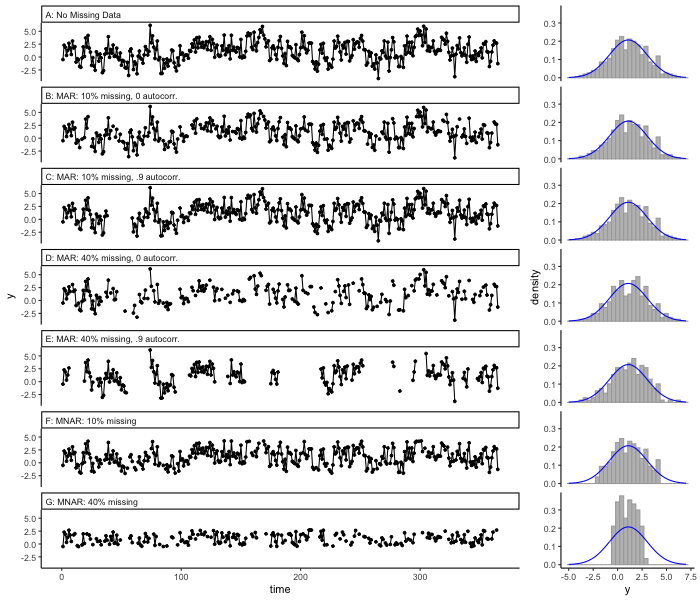
\includegraphics[width = 0.85\textwidth]{Figures/CompareMissingnessTypes_fig.png}
     \caption{An example time series demonstrating different types and amounts of missing data. The left column shows the same time series with different amounts and types of missingness and right column shows the distribution of data points in each resultant time series. A. Complete time series with no missing data. Rows B through E show the time series with 10\% (B and C) or 40\% (D and E) of data missing completely at random (MCAR), with either low autocorrelation in missing data (B and D) or high autocorrelation (C and E). Rows F and G show the time series with data missing not at random (MNAR) for 10\% missing data (F) and 40\% missing data (G).}
     \label{fig:missingtypes}
 \end{figure}

 \begin{figure}
     \noindent\includegraphics[width = 0.85\textwidth]{Figures/MockedUpFigures/heatmap_GaussianMCAR_all.png}
     \caption{Median error of parameter recovery, median absolute error, and model coverage of $\phi$ and $\beta$, depending on the proportion of missing data and autocorrelation in missingness for each of five missing data approaches, using simulated, real-valued datasets with data missing completely at random (MCAR).}
     \label{fig:GaussianMCARheatmapALL}
 \end{figure}

  \begin{figure}
         \noindent\includegraphics[width = 0.85\textwidth]{Figures/MockedUpFigures/heatmap_PoissonMCAR_all.png}
     \caption{Median error of parameter recovery, median absolute error, and model coverage of $\alpha$ and $r$, depending on the proportion of missing data and autocorrelation in missingness for each of five missing data approaches, using simulated time series of counts with data missing completely at random (MCAR). Note that coverage is not shown for the Expectation Maximization approach, since most implementations of this method do not include estimates of standard error.}
     \label{fig:PoissonMCARheatmapALL}
 \end{figure}
 
%\subsection{Bias due to endogeneity}

%It is well known that the ordinary least squares estimator (OLS) of the autoregressive coefficients in an AR($p$) model is biased. To see this, consider a simple AR(1) model with mean zero and variance of the innovations $\sigma^2$. The model can be written as
%$$
%y_t = \phi y_{t-1} + \epsilon_t
%$$
%where $\epsilon_0, ..., \epsilon_n \overset{iid}{\sim} \mathcal{N}(0, \sigma^2)$ and $\phi$ is the autoregressive coefficient. The OLS estimator of $\phi$, $\hat{\phi}$ is obtained by regressing observations $y_1,...,y_n$ against $y_0,...,y_{n-1}$. Thus, the OLS estimator can be written as
%\begin{equation*}
%    \begin{aligned}
%        \hat{\phi} &= \frac{\sum_{t=1}^n y_t y_{t-1}}{\sum_{t=1}^n y_{t-1}^2}\\
%        &= \frac{\sum_{t=1}^n (\phi y_{t-1} + \epsilon_t) y_{t-1}}{\sum_{t=1}^n y_{t-1}^2}\\
%        &= \frac{\sum_{t=1}^n (\phi y_{t-1}^2 + \epsilon_t y_{t-1})}{\sum_{t=1}^n y_{t-1}^2} \\
%        &= \phi \frac{\sum_{t=1}^n y_{t-1}^2}{\sum_{t=1}^n y_{t-1}^2} + \sum_{t=1}^n \frac{y_{t-1}}{\sum_{t=1}^n y_{t-1}^2} \epsilon_t\\
%        &= \phi + \sum_{t=1}^n \frac{y_{t-1}}{\sum_{t=1}^n y_{t-1}^2} \epsilon_t.
%    \end{aligned}
%\end{equation*}
%Taking the expectation,
%\begin{equation*}
%    \mathbb{E}(\hat \phi) = \phi + \mathbb{E}\left(\sum_{t=1}^n \frac{y_{t-1}}{\sum_{t=1}^n y_{t-1}^2} \epsilon_t \right)
%\end{equation*}
%we see that, because the sum in the denominator of the second term in the expectation, $\sum_{t=1}^n y_{t-1}^2$, is not independent of $\epsilon_t$ (if $\epsilon_t$ is large and positive, the sum in the denominator will also increase), the ``covariate" we use is \textit{endogenous}, meaning it is not independent of the errors. The negative correlation between $\epsilon_t$ and the reciprocal of sum $\sum_{t=1}^n y_{t-1}^2$ results in a downward-biased estimator of $\phi$ (i.e, closer to zero). 




\newpage


\end{document}

\section{Supplemental Information}
Figures: 
\textbf{Potential additional figures in Supplement}

* Supp. Fig. 1: Multi-panel plot of raw GPP, light, and discharge time series

* Supp. Fig. 2: Plot of raw population time series 
\begin{figure}[h]
    \centering
    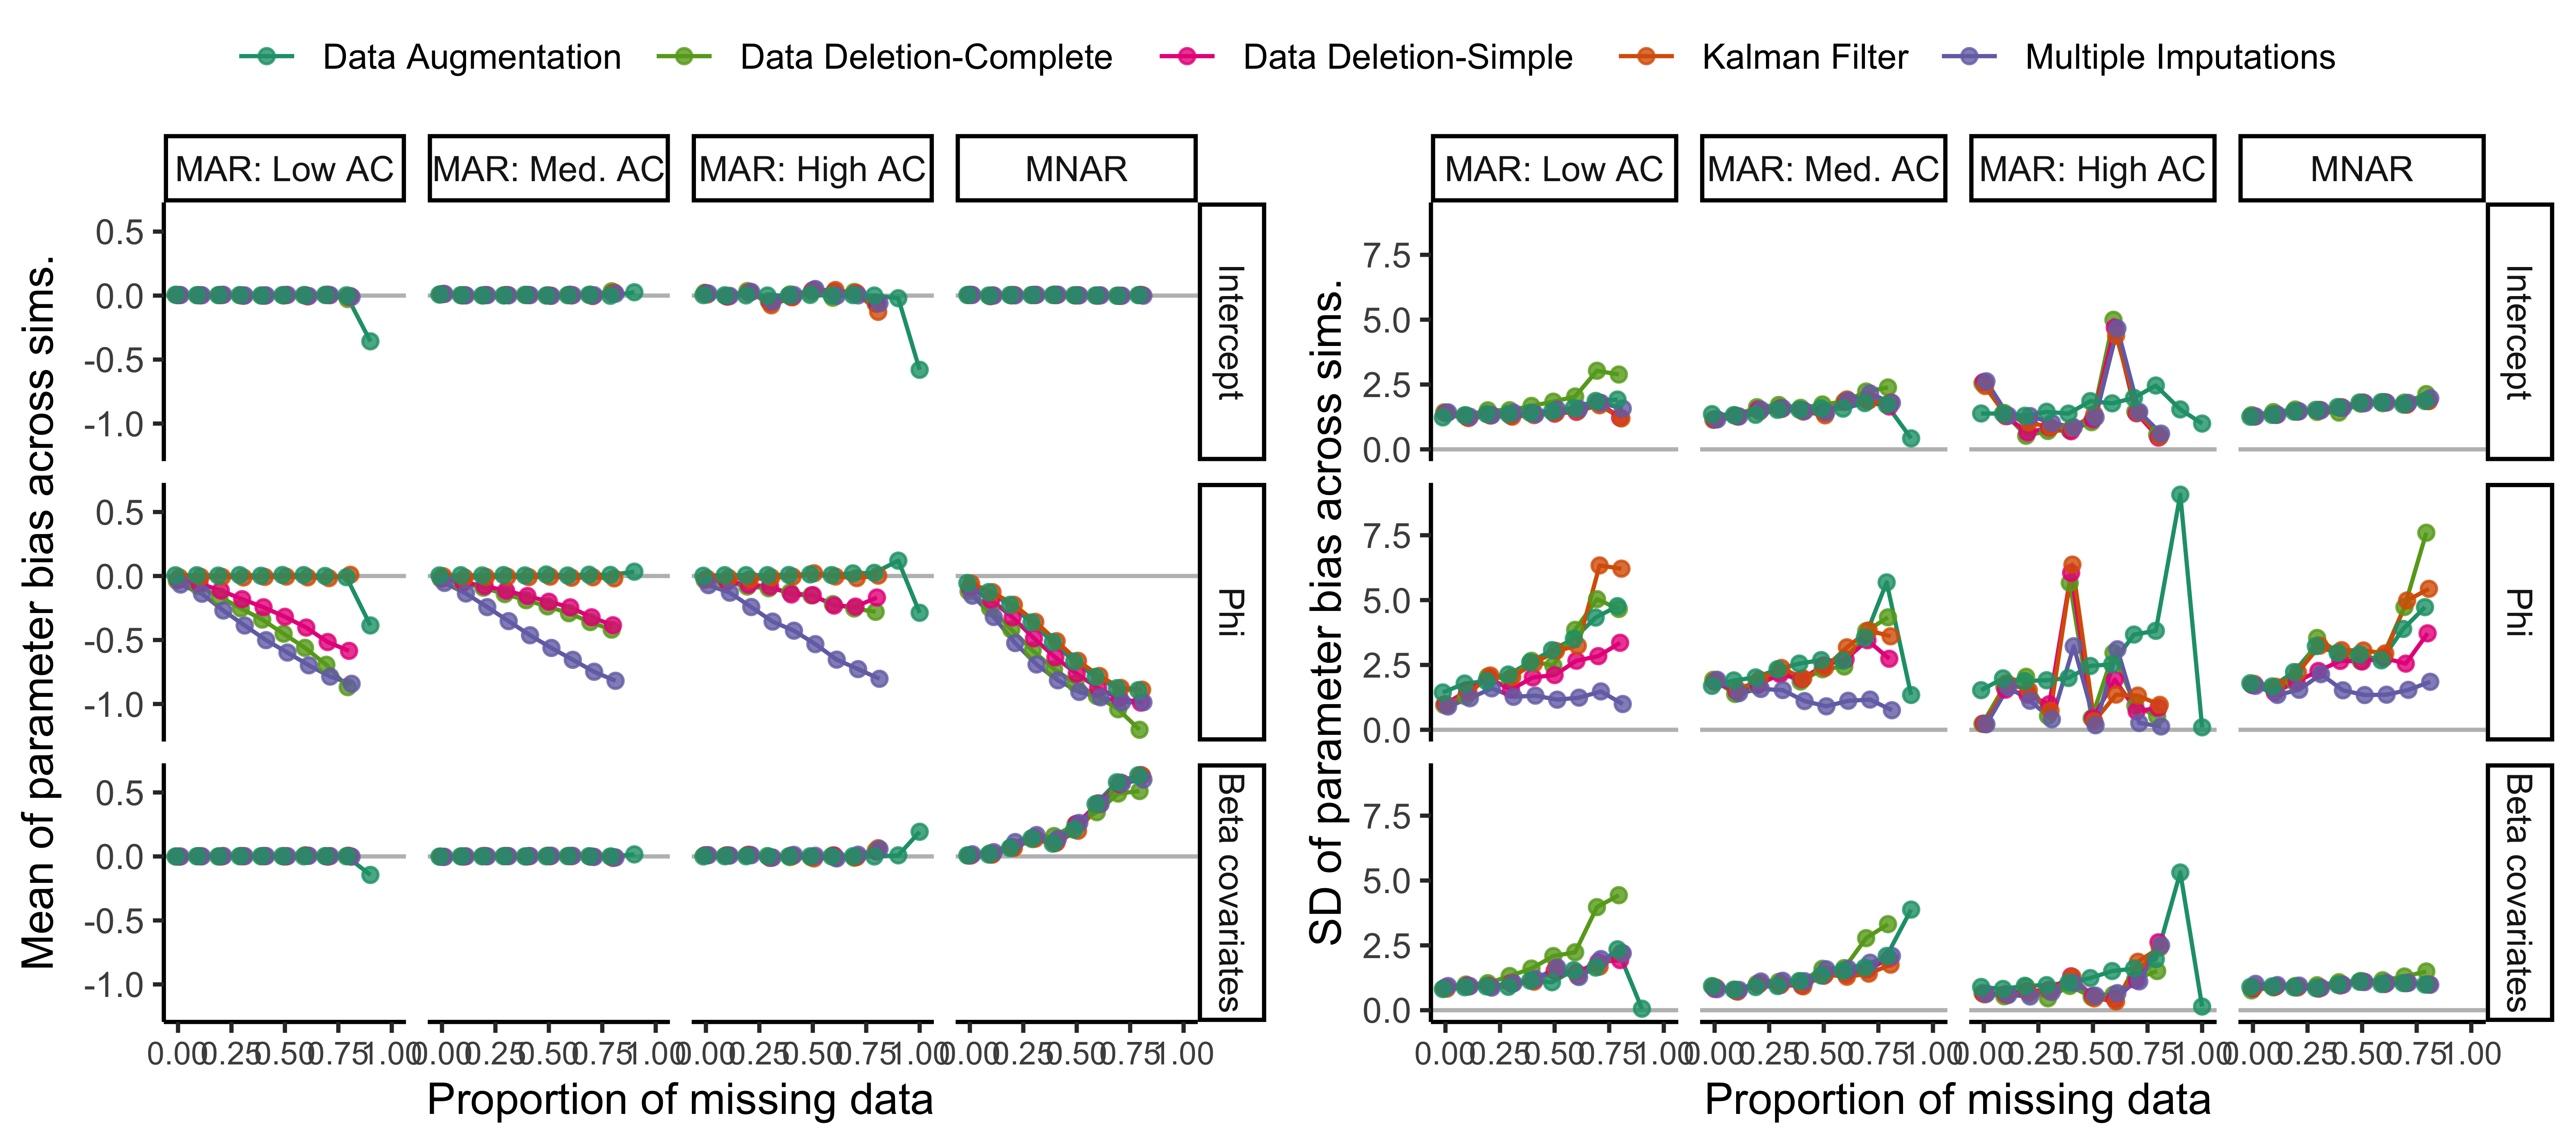
\includegraphics[width=\linewidth]{Figures/parameterRecovery_sim_Guassian_medsSD.png}
    \caption{Medians and standard deviations of parameter estimate recovery using simulated Gaussian datasets--complete x-axis}
    \label{fig:GaussianParamRecov_medSD_all}
\end{figure}


\begin{figure}
    \noindent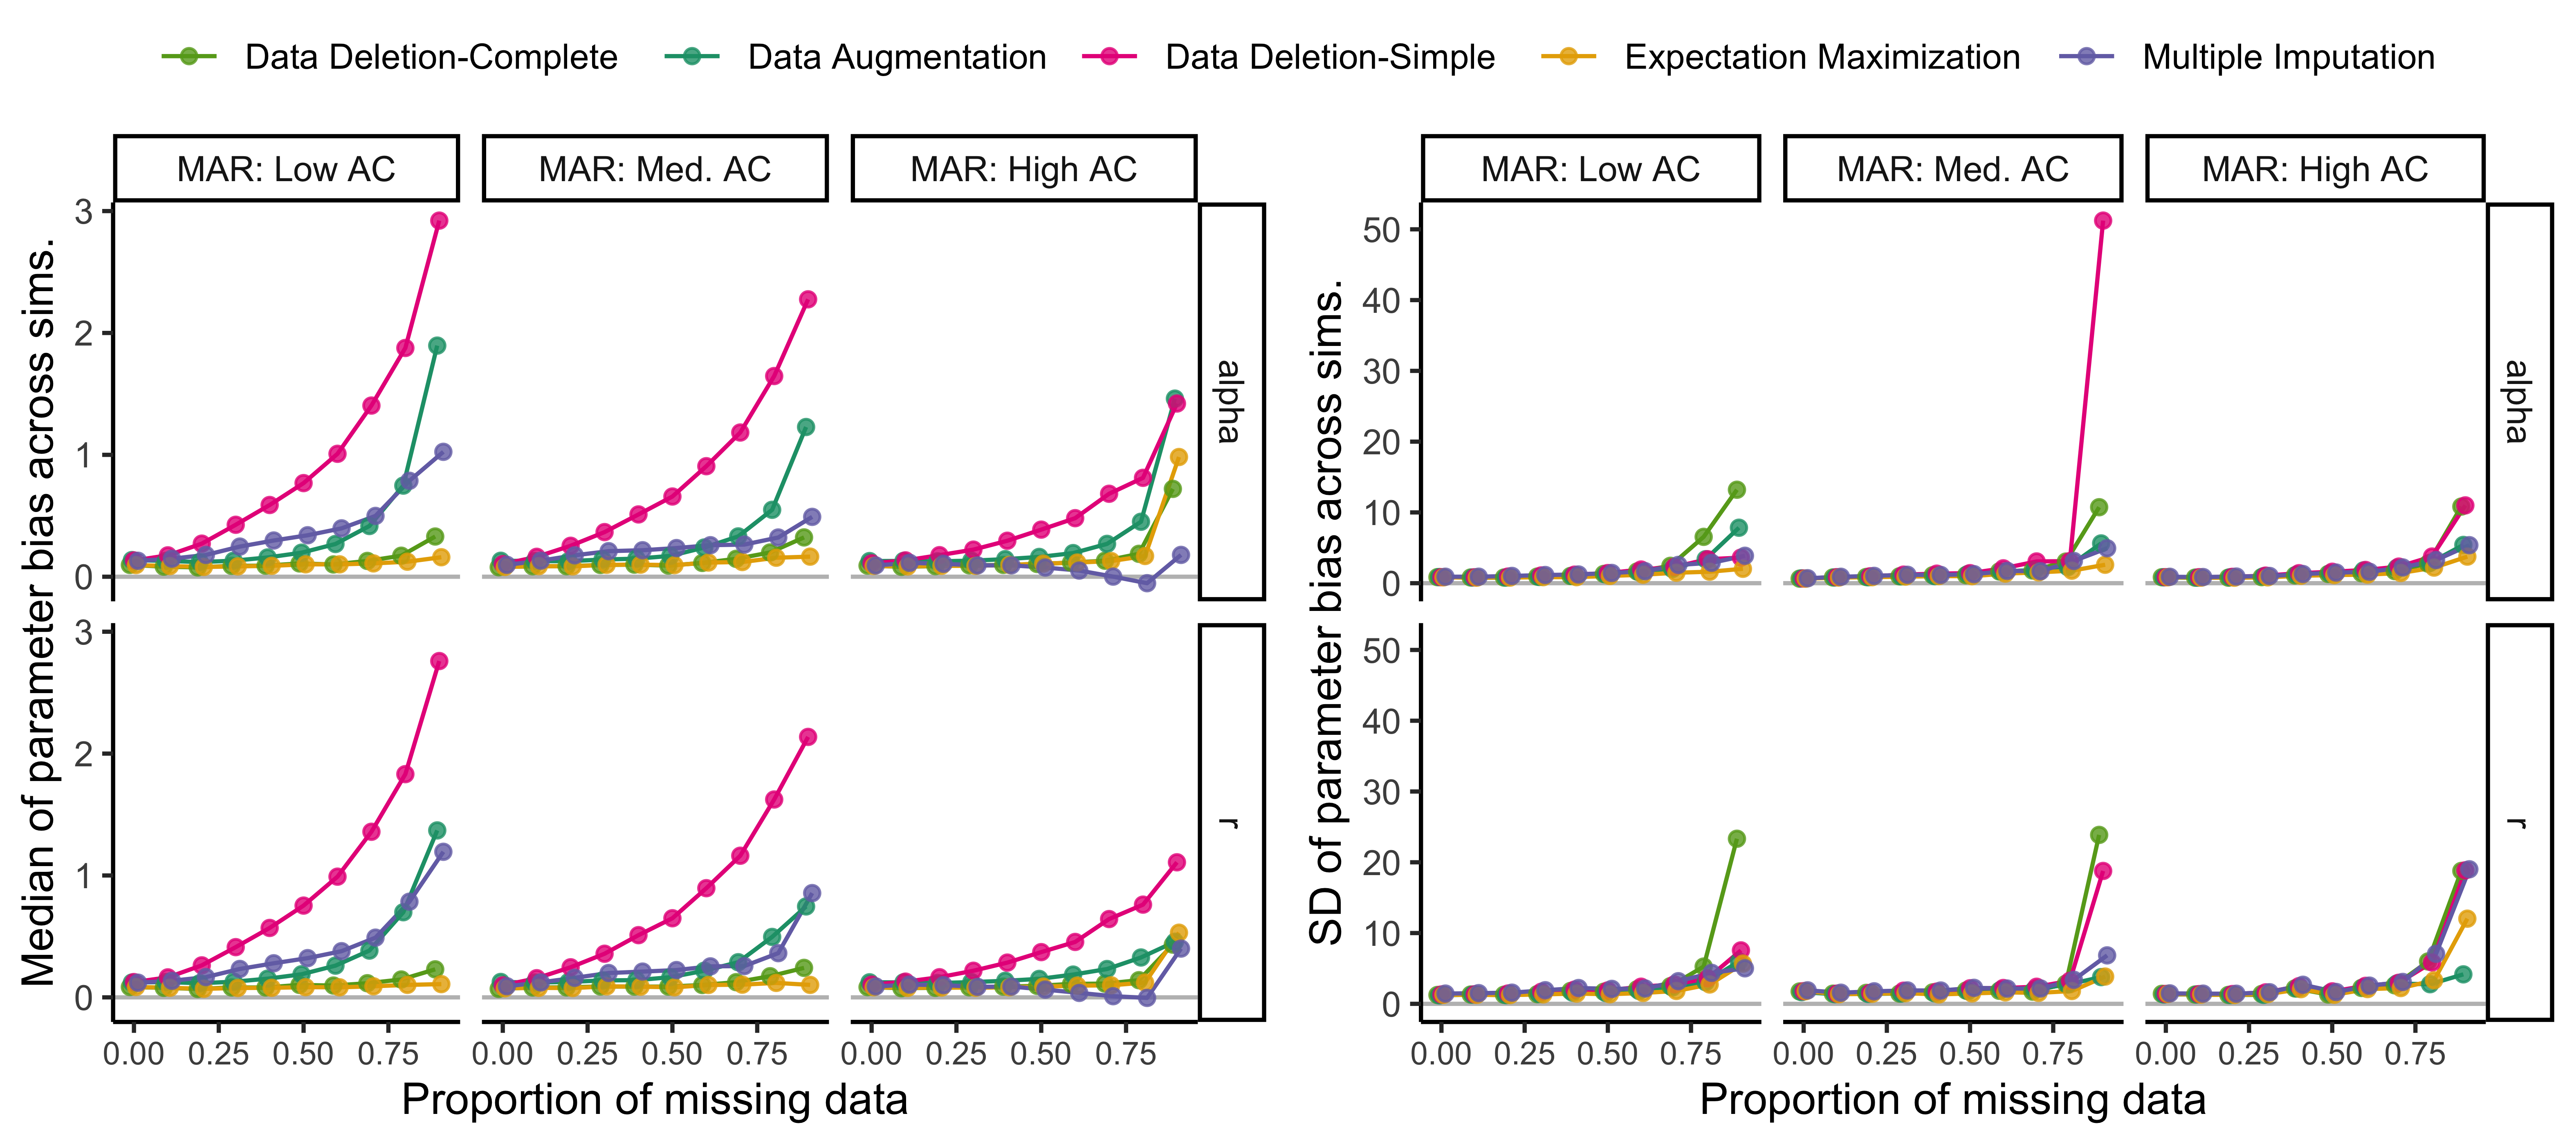
\includegraphics[width = \textwidth]{Figures/parameterRecovery_sim_Poisson_medsSD.png}
    \caption{Medians and standard deviations of parameter estimate recovery using simulated Poisson datasets--complete x-axis}
    \label{fig:PoissonParamRecov_medSD_all}
\end{figure}

\clearpage

\begin{figure}
    \centering
    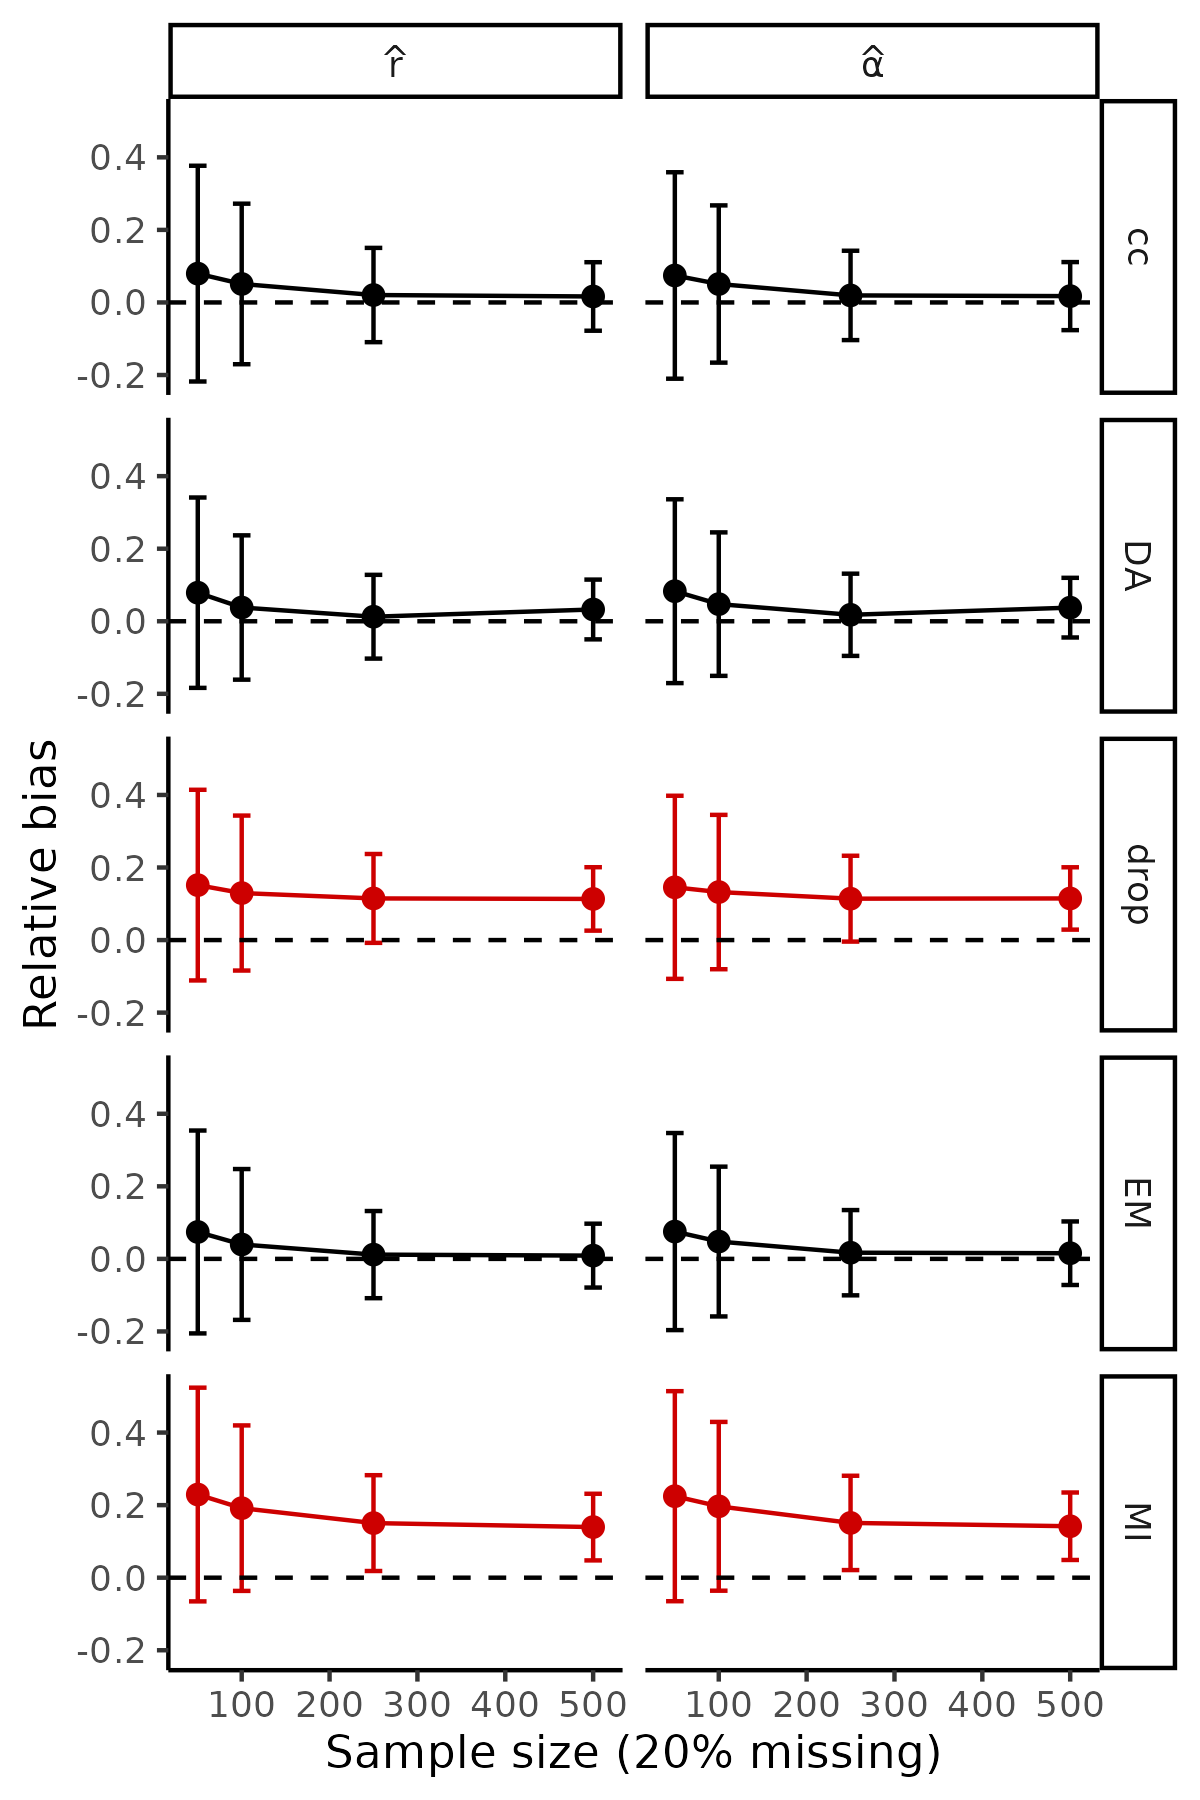
\includegraphics[width=0.75\linewidth]{Figures/bias_checks_ricker.png}
    \caption{Results from simulation experiments with 250 parameter sets at each of four sample sizes to assess estimator bias with increasing sample sizes. All estimators are small-sample biased, but only the simple data deletion (\textit{drop}) method and the multiple imputation approach using package \texttt{Amelia} retain substantial bias at larger sample sizes. Error bars show plus and minus one standard error of the estimator.}
    \label{fig:bias-checks}
\end{figure}

%%%%%%%%%%%%%%%%%%%%%%%%%%%%%%%
\end{document}
%%%%%%%%%%%%%%%%%%%%%%%%%%%%%%%
